\documentclass[12pt,a4paper]{report}
%\usepackage[a4paper, total={6in, 8in}]{geometry}
\usepackage{geometry}
 \geometry{
 top=25mm,
 }
 \usepackage{mathtools}
\usepackage{amsmath}
%\usepackage[showframe]{geometry}
\usepackage{titlesec}
%\usepackage{titletoc,tocloft}
\usepackage[english]{babel}
\usepackage[T1]{fontenc}
\usepackage{mathptmx}
%\usepackage{newtxmath,newtxtext}
%\usepackage[utf8x]{inputenc}
\usepackage{amsmath}
\usepackage{graphicx}
\graphicspath{ {images/} }
\usepackage[colorinlistoftodos]{todonotes}
\usepackage[yyyymmdd]{datetime}
\usepackage{tikz}
\usetikzlibrary{calc}
\usepackage{sectsty}
\usepackage{float}
%\usepackage[tocflat]{tocstyle}
%\usetocstyle{standard}
%\usepackage[table,xcdraw]{xcolor}
\sectionfont{\fontsize{18pt}{15}\selectfont}
\usepackage{tocloft}
\usepackage{subcaption}
%\renewcommand{\cftsecleader}{\cftdotfill{\cftdotsep}}
%add page no
%\addtocontents{toc}{{\bfseries \hfill Page No.\bigskip\par}}

%\setlength{\cftsubsecindent}{2cm}
%\setlength{\cftsubsubsecindent}{4cm}

\setcounter{secnumdepth}{4}

\titleformat
{\chapter} % command
[display] % shape
{\bfseries\Large} % format
{\centering Chapter \thechapter} % label
{0.5ex} % sep
{
%    \rule{\textwidth}{1pt}
%    \vspace{1ex}
\Large 
    \centering
    \MakeUppercase
} % before-code
\titlespacing*{\chapter}{0pt}{-50pt}{30pt}


%\tableofcontents


\begin{document}
\pagenumbering{roman}
\linespread{1.3}
%\addcontentsline{toc}{section}{Unnumbered Section}\
\addcontentsline{toc}{section}{\textbf{Approval}}
\fontsize{13pt}{12}\selectfont{Approval of the Department of Electronic \& Telecommunication Engineering}\\[2cm]

\begin{table}[h]
\begin{tabular}{cc}
 & \hspace{8cm}..........................................                                                                               \\
 & \begin{tabular}[c]{@{}c@{}}\hspace{8cm}Head, Department of Electronic \&\\ \hspace{8cm}Telecommunication Engineering\end{tabular}
\end{tabular}
\end{table}
\vspace{2.5cm}
\noindent This is to certify that I/we have read this project and that in my/our opinion it is fully adequate, in scope and quality, as an Undergraduate Graduation Project.\\[1cm]
Supervisors:\\[0.5cm]
Dr. Ranga Rodrigo\\[1cm]
Signature: ......................\\[1cm]
Dr. Ajith Pasqual\\[1cm]
Signature: ......................\\[1cm]
Dr. Peshala G. Jayasekara\\[1cm]
Signature: ......................\\[2cm]
Date: ......................\\


\newpage
\addcontentsline{toc}{section}{\textbf{Declaration}}
\begin{center}
\fontsize{18pt}{12}\selectfont{\textbf{Declaration}}
\end{center}
\fontsize{12pt}{12}\selectfont
This declaration is made on October 5, 2017.\\[1cm]
\textbf{Declaration by Project Group}\\
We declare that the dissertation entitled People Counting and Tracking with Xilinx ZC702 Evaluation Kits and the work presented in it are our own. We confirm that:
\begin{itemize}
\item this work was done wholly or mainly in candidature for a B.Sc. Engineering degree at this university,
\item where any part of this dissertation has previously been submitted for a degree or any other qualification at this university or any other institute, has been clearly stated,
\item where we have consulted the published work of others, is always clearly attributed,
\item where we have quoted from the work of others, the source is always given. With the exception of such quotations, this dissertation is entirely our own work,
\item we have acknowledged all main sources of help.
\end{itemize}
\vspace{1cm}
\begin{table}[h]
\begin{tabular}{cccc}
........................... &&& \hspace{5cm}...........................  \\
Date                        &&& \hspace{5cm}R.V.C.N Abeyrathne (130008K) \\[1cm]
                            &&& \hspace{5cm}...........................  \\
                            &&& \hspace{5cm}D.L Dampahalage (130093M)    \\[1cm]
                            &&& \hspace{5cm}...........................  \\
                            &&& \hspace{5cm}H.A.S.P Gunasekara (130183N) \\[1cm]
                            &&& \hspace{5cm}...........................  \\
                            &&& \hspace{5cm}W.M.D.K Weerakoon (130633V) 
\end{tabular}
\end{table}
\newpage
\noindent \textbf{Declaration by Supervisors}\\[0.5cm]
We have supervised and accepted this dissertation for the submission of the degree.\\[1cm]
\begin{table}[h]
\begin{tabular}{cc}
........................... & \hspace{5cm}........................... \\
Dr. Ranga Rodrigo           & \hspace{5cm}Date                        \\[1cm]
........................... & \hspace{5cm}........................... \\
Dr. Ajith Pasqual           & \hspace{5cm}Date                        \\[1cm]
........................... & \hspace{5cm}........................... \\
Dr. Peshala G. Jayasekara   & \hspace{5cm}Date                       
\end{tabular}
\end{table}
\newpage
\addcontentsline{toc}{section}{\textbf{Abstract}}
\begin{center}
\fontsize{18pt}{18}\selectfont{\textbf{Abstract\\[1cm]
People Counting and Tracking with Xilinx ZC702\\
Evaluation Kits}}\\[0.5cm]
\fontsize{12pt}{12}\selectfont{Group Members: R.V.C.N Abeyrathne, D.L Dampahalage, H.A.S.P Gunasekara, W.M.D.K Weerakoon}\\[0.25cm]
Supervisors: Dr. Ranga Rodrigo, Dr. Ajith Pasqual, Dr. Peshala G. Jayasekara
\end{center}
\textit{Keywords}: FPGA,ZYNQ-7000, people counting, multi-camera, multiple people tracking, particle filters, gaussian mixture models\\[0.5cm]
In the contemporary society making correct decisions is vital for any business organization to stay on par with competitors. For that intent identifying and understanding the
customers is a must. Tapping into the customers$'$ subconscious is the preeminent way of making correct business decisions and for that an organization should track and analyze customer behavior.\\
As a solution to this problem, we propose a scalable multi-camera people tracking system for a large department store like environment. The main focus of this project is to implement an end to end system for multi-camera people tracking with business intelligence.
Novelty of this system from contemporary multi-camera people tracking systems is the introduction of leaf node processing, where part of the processing is done in a hardware system close to the camera. By this way we could achieve the scalability required for a large department store like environment and reduce bandwidth usage in such systems.\\
This proposed system comprises of leaf nodes, central server and the web server. Leaf nodes are integrated close each camera. We use Zynq SoCs for leaf nodes and these devices read video frames from the cameras, detects people for each frame using GMM based background subtraction, calculate color histogram features for each detected person and sends the bounding boxes and features to the server using UDP.\\
A central server will receive this information from each leaf node and do people tracking by using particle filters and hungarian algorithm for data association. Multi-camera tracking is also achieved by means of homography based method and a graph algorithm. Real time tracking and heatmaps are generated in the server GUI.\\
Finally business intelligence software hosted in a web server, where real time people tracking for the whole store, heatmaps for desired time period, people count graphs for desired time period and real time people count graphs are implemented.\\
Therefore by the introduction of leaf node processing we achieve a scalable system since the processing power required at the central server is reduced. We achieve a low power system for leaf nodes by using Zynq SoCs and we reduce the bandwidth usage since we only send the bounding boxes and features for tracking to the server.


\newpage
\addcontentsline{toc}{section}{\textbf{Acknowledgments}}
\begin{center}
\fontsize{18pt}{18}\selectfont{\textbf{Acknowledgments}}
\end{center}
\vspace{1cm}
We would like to express our deepest appreciation and sincere gratitude to our project supervisors, Dr. Ajith Pasqual, Dr. Ranga Rodrigo and Dr. Peshala Jayasekara of Department of Electronic and Telecommunication Engineering of University of Moratuwa, for their guidance and constant supervision as well as for providing necessary information regarding the project.\\
\par We would like to thank ParaQum Technologies for their guidance and support given to us during the project.
We are indebted to our final year project coordinator, Dr. Anjula Silva for his counsel regarding the project.
We would also like to take this opportunity to thank Ms. Salgado for her advices on compiling a finer report.
We would like to acknowledge with much appreciation the non-academic staff of the department who gave us their fullest support in providing necessary laboratory facilities.\\
\par Finally, our thanks and appreciations also goes out to our batch mates who helped in numerous ways to make this endeavor a success.
\newpage
\titleformat*{\section}{\centering\bfseries\Large}
\tableofcontents
\titleformat*{\section}{\bfseries\Large}
\newpage
\addcontentsline{toc}{section}{\textbf{List of Figures}}
\listoffigures
\newpage
\addcontentsline{toc}{section}{\textbf{List of Tables}}
\listoftables
\newpage
\addcontentsline{toc}{section}{\textbf{Acronyms and Abbreviations}}
\begin{center}
\fontsize{18pt}{18}\selectfont{\textbf{Acronyms and Abbreviations}}
\end{center}
\vspace{0.75cm}

\begin{table}[H]
\centering
\begin{tabular}{ll}
FPGA & Field Programmable Gate Array \\
GMM & Gaussian Mixture Models\\
PCA & Principal Component Analysis \\
YOLO                     & You Only Look Once                                \\
IP                       & Intellectual Property                             \\
SoC                      & System on Chip                                    \\
RTL                      & Register Transfer Level                           \\
AXI                      & Advanced eXtensible Interface                      \\
HLS                      & High Level Synthesis                              \\
UIO                      & Userspace Input/Output                            \\
REST                     & Representational State Transfer                   \\
API                      & Application Programming Interface                 \\
AJAX                     & Asynchronous JavaScript ond XML                   \\
JSON                     & JavaScript Object Notation                        \\
UDP                      & User Datagram Protocol                            \\
TCP                      & Transmission Control Protocol                     \\
URL                      & Uniform Resource Locator                          \\
SDRAM                    & Synchronous Dynamic Random Access Memory          \\
DDR                      & Double Data Rate                                 
\end{tabular}
\end{table}
\newpage
\pagenumbering{arabic}
\setcounter{page}{1}

\chapter{\textbf{Introduction}}

Nowadays retail stores are very popular among people. Even in Sri Lanka, retail stores like Cargills Food City and House of Fashion are visited by at least few hundreds of customers daily. In these type of retail stores, one of the factors that are used to measure the effectiveness of an advertisement or the popularity of store is the conversion rate. This number represents the percentage of the people actually bought something out all the people that visited the store. Usual way of calculating the conversion rate is by counting the people coming to the store and checking out at one of the counters. It is impractical to do this manually in a large retail store environment. Other than calculating the conversion rate, various business decisions could be made for the betterment of the store by analyzing customer behaviour. \\\\
Enhancing customer experience by rearranging the store structure, efficiently allocating staff to high density areas, understanding Traffic trends and identify "opportunity hours" and schedule labor hours accordingly to optimize service levels are some of such business decisions In order to assist making business decisions, large-scale retail stores need to count and track people using a number of ceiling-mounted cameras. In such environment it is hard to keep track of customer behavior separately using a manual system.\\\\
Identifying the history of  customers and understanding the customer density inside the areas of the department store can be critical for financial and business decisions. However if a system is in place which counts and tracks the customers inside the store and generates basic intelligence to the managerial level, it can expedite the decision making process. This project is aimed at developing such a system. We have implemented a people tracking and counting system adaptable to any large scale store structure which is able to process multiple video streams obtained through separate cameras mounted on the store and generate business intelligence.\\\\
There have been several systems which handle multi camera people tracking introduced in the past decade. All these systems incorporate a central server which will receive all the frames from all the cameras to handle the people detection and tracking tasks real-time. Major drawback of these systems is the scalability. When the number of cameras increase, the bandwidth usage for sending video frames to the central server will be increased and the processing power required at the central server will increase. This raises the requirement for processing video frames close to the camera which is defined as leaf node processing. \\\\
The scope of this project is to implement a scalable end to end system for Multi-Camera People Tracking utilizing a Zynq SoC for leaf node processing. Thereby we use an FPGA + ARM processor for leaf node processing, a central server for multi-camera people tracking and a web server for generating business intelligence.\\\\
In this proposed system by using a FPGA + ARM processor we have achieved leaf node processing of people detection at a lower power and also enable the scalability and lower bandwidth requirement. \\\\
People Detection in FPGA is an aspect that has been researched by many over the
years. For example [2] suggests a FPGA based embedded platform for people detection using Gaussian Mixture Models and [3] suggests a similar system for people detection using Histogram of Features.\\\\
Multi-Camera People Tracking systems is also a field which has been researched over the years. [4] suggests a multi-camera surveillance system implemented with background subtraction for detection and color features for tracking. [6] suggests another multi camera people tracking system which uses particle filters for tracking on the ground plane.
\chapter{Literature Review}
In this project main focus was to implement an end to end system for Multi-Camera People Tracking System and to use this system to generate business intuition. As explained earlier we use the technique of leaf node processing to achieve a scalable, low power, low bandwidth required system.\vspace{0.3cm} 

There are several challenging tasks in implementing this system. One is people detection in FPGA. There are various ways to achieve this. One way is to use a blob detection algorithm as used by Vicente, Alfredo Gardel, et al. [1] in 2009.They have done background subtraction followed by contour detection to select head candidates for videos obtained using overhead cameras and they have implemented people detection part in a low cost FPGA (spartan3).\vspace{0.3cm}

Feature based methods are also another way to do people detection. In these methods a set of features are calculated around a window and some kind of machine learning algorithm is used to train a classifier that can classify each window into "contains a person" and "not contains a person". One such method is Histogram Oriented Gradient (HoG) based method suggested by Dalal, Navneet, and Bill Triggs. [2] in 2005. A variation of HoG is implemented on FPGA by Negi, Kazuhiro, et al. [3] in 2011.\vspace{0.3cm}

Another approach that can be used for people detection is to utilize a neural network. If we can come up with a suitable neural network architecture, this method has the potential to outperform all the other methods mentioned earlier. There are several open source implementations of such architectures available. One such architecture is given by Redmon, Joseph, et al. [4] in 2016. Their work has made a huge leap in object detection space. Due to its success their architecture is utilized by many people. Challenge though in using this approach is the complexity of implementing a convolutional neural network in an FPGA.  Implementing a CNN architecture in FPGA with the available resources and to achieve real time processing is an immense challenge. \vspace{0.3cm}

We used a background subtraction based method for people detection in the proposed system. Though we considered using either HoG or CNN, as our focus was to implement the end end architecture for multi-camera people tracking with leaf node processing, background subtractions deemed to be a feasible solution. We could improve the existing system by implementing either HoG or CNN as a future improvement.\vspace{0.3cm}

Other major challenge we have is people tracking based on our detections. There are many traditional approaches to this such as tracking using kalman filter and assigning detections to tracks using the Hungarian algorithm. But multi target tracking also can be formulated as a discrete-continuous optimization problem [5]. Andriyenko, Anton, Konrad Schindler, and Stefan Roth [5] in 2012 have considered data association as a discrete optimization problem with label costs. And they have posed trajectory estimation as a continuous fitting problem with closed form solutions. And there method has performed well on some known data sets.\vspace{0.3cm}

Other major challenge that we face is, how to extend multiple target tracking into a multi camera framework. There are some research papers discussing this issue. Tang, Nick C., et al. [6] in 2015 suggest a two pass regression framework to solve this challenge. First pass regression predicts the people count based on the features calculated from intra-camera video frames. And then the second pass is based on the conflicts between the prediction derived from multiple views. They have formulated this as a transfer learning problem. Yang, Tao, et al. [7] in 2007 discusses another method to do this. In this approach first they do single camera tracking and they transform these tracked paths into a global coordinate system. Then by using their multi camera handoff algorithm, they can track people across multiple cameras. Here they calculate a match score for an object appearing in a camera under overlapping or non overlapping conditions for all tracks under all cameras. The track having the maximum score is selected.\vspace{0.3cm}

By going through the available literature we were able to get an insight of the scope of our project. We identified some potential solutions for the challenges we have. We were also able to identify that implementing the overall system architecture for multi-camera people tracking with leaf node processing will be a novel contribution. 


\chapter{Methodology}
\section{Introduction}
In this project we have designed and implemented an end to end multi camera people counting and tracking system based on Xilinx ZC702 development board. In this implementation we have considered the possibility of using leaf node processing to develop a scalable solution for multi camera people tracking. In this chapter we present the underline methodology of our system in detail.
In order to give the reader a gradual walkthrough of our project we will explore each component of our system separately. First we will give an overview of the basic system. Then we will explore in detail the each component of our system. 
\section{Scope}
The main components of the project that makes the scope is as follows.
\begin{itemize}
\item People Detection feature extraction\\
This involves reading image frames from the camera and extracting the features
required for people detection. This computation will be done in the Programmable
Logic (PL) of Zynq ZC702 Evaluation Kit.
\item Writing Linux Kernel drivers for controlling PL IP cores.\\
Writing Linux Kernel drivers are required to control the IP cores from the software end.
\item Communication with the backend server \\
Calculated features for each image frame will be sent to the backend server through Ethernet for the rest of the processing.
\item Multi- Camera People Tracking \\
Multi-Camera people tracking will be done in the backend server using the features sent through each of the cameras.


\end{itemize}
\section{Overall Architecture}
\begin{figure}[H]
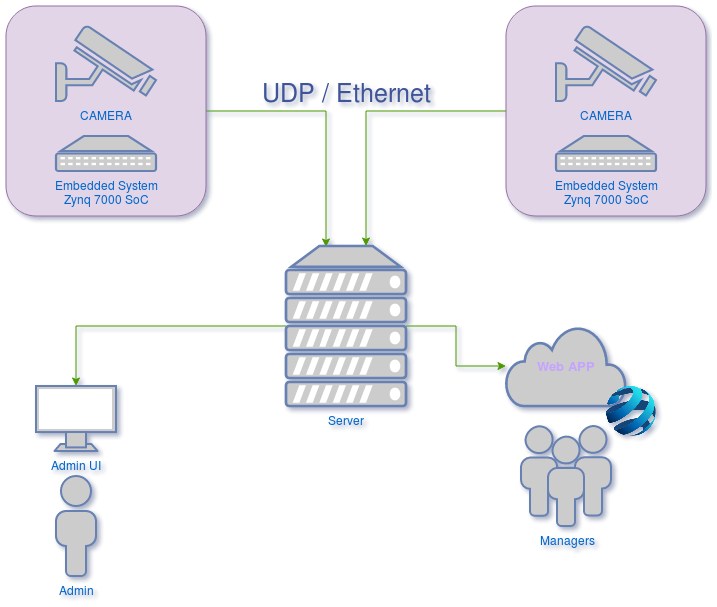
\includegraphics[width=10cm]{overall_block.png}
\centering
\caption{Overall block diagram of the end-to-end system}
\label{overall}
\end{figure}

Figure \ref{overall} shows the overall architecture of our system. It mainly consist of 3 components, namely,
An embedded system closer to the camera (Leaf node)
People tracking applications running on a server 
Business intelligence generation and displaying interfaces. 

We will explore each of the above components separately in the following sections.

\section{Embedded System (Leaf Node)}
Generally the term 'leaf node' is used for a system placed at the edge or bottom of a hierarchical network (of systems). In our system, leaf node is the embedded system connected to the camera.  \\\\
This embedded system  is responsible for capturing live video frames from the camera and preprocessing before sending into the central server. Objective of preprocessing on the leaf node is to reduce the required bandwidth of the network to send information (video in this case) to the central server and to reduce the processing done one the central server in a scalable manner. 
In a large system consisting of few hundreds of cameras, reduction of the bandwidth required and the processing power of the central system for each camera makes a big difference in the central system processing and bandwidth requirements, making the system more scalable.  
\\\\
In our prototype system, leaf node consists of a web camera connected to a Xilinx ZC702 development board and its responsible for doing people detection of the live video feed and feature calculation of the detected people. Implementations of the people detection and feature calculation algorithms are explained in detail in later sections. These calculated features of the detected people are then sent to the central server via a custom application layer protocol based on User Datagram Protocol (UDP) / Internet Protocol (IP) over Ethernet.
\\\\
Following sections provide an overview about the feature of Xilinx ZC702 board and ZYNQ-7000 All Programmable (AP) System on Chip (SoC).

\subsection{Xilinx ZC702 Board}
Xilinx ZC702 board, shown in Figure \ref{board}, is a development board manufactured by Xilinx targeting embedded hardware (FPGA) design development. This board consists of a ZYNQ-7000 AP SoC with various other peripherals. Key features and peripherals of Xilinx ZC702 is listed below.




\begin{itemize}
\item Zynq-7000 SoC
\item 1GB DDR3 Component Memory
\item Enabling serial connectivity with USB OTG, UART, IIC, CAN Bus
\item Ethernet which supports 10-100-1000 Mbps transfer rates
\item HDMI interface
\item FPGA Mezzanine Card (FMC) interface
\item Onboard Secure Digital (SD) card reader
\end{itemize}


\begin{figure}[H]
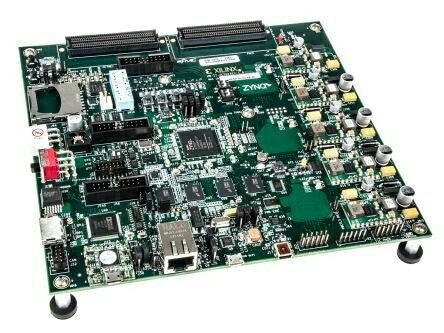
\includegraphics[width=10cm]{zc702.jpg}
\centering
\caption{Xilinx ZC702 Development Board}
\label{board}
\end{figure}


Features of the onboard ZYNQ-7000 SoC and usage of it in our project is explained in following sections.

\subsection{ZYNQ-7000 SoC}
ZYNQ-7000 SoC consists of a Xilinx XC7Z020-CLG484-1 FPGA and two ARM Cortex-A9 core processors. Block diagram in figure \ref{zynq} shows how the Programmable Logic and the Processing System is connected inside the ZYNQ-7000 SoC.

\begin{figure}[H]
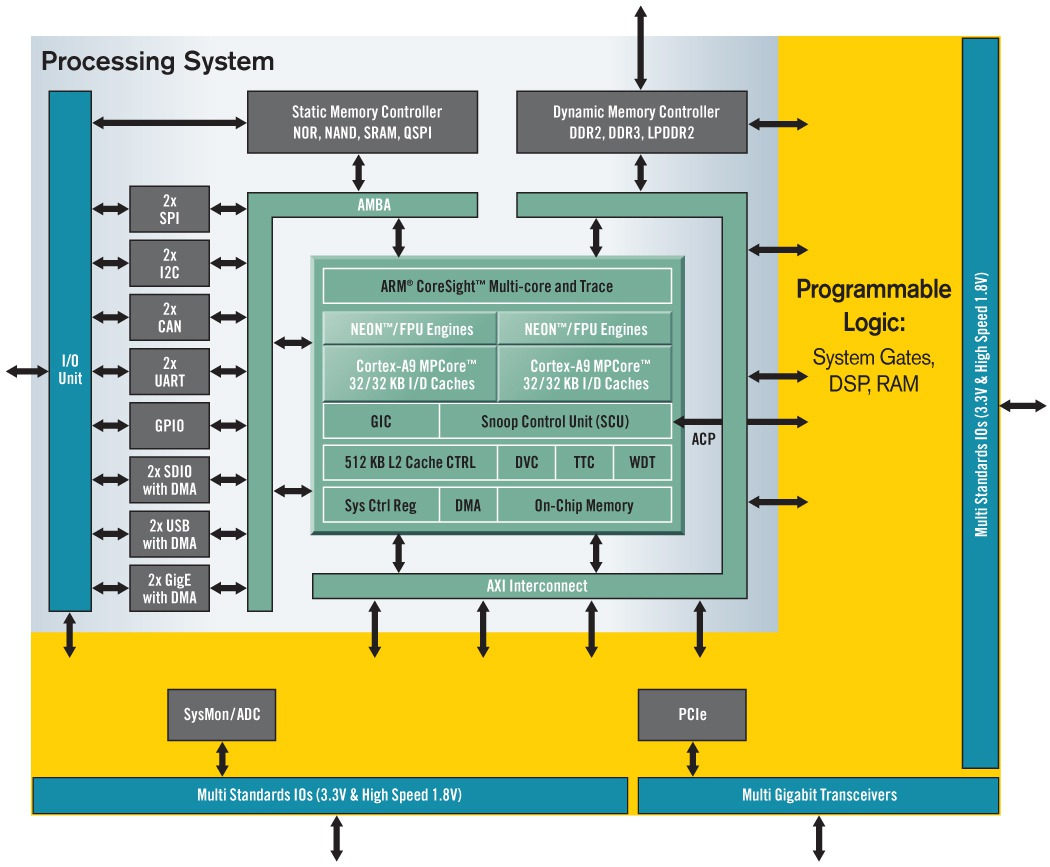
\includegraphics[width=10cm]{zynq.jpg}
\centering
\caption{Internal architecture of ZYNQ-7000 SoC}
\label{zynq}
\end{figure}

In our implementation, we have installed a lightweight Linux distribution on dual ARM processors in ZYNQ-7000 SoC. Reasons for installing Linux and its usage is explained in a latter section.


\subsection{Design Flow for ZYNQ-7000 based Embedded System}
We used the standard Xilinx toolchain for developing an embedded system for designing and implementing our leaf node system. Figure \ref{design} shows a block diagram of the design flow with the design tools we used.

\begin{figure}[H]
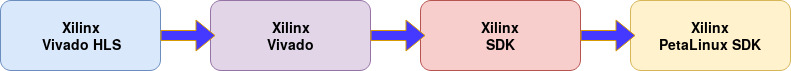
\includegraphics[width=13cm]{design.jpg}
\centering
\caption{Design flow block diagram for ZYNQ-7000 based embedded system}
\label{design}
\end{figure}

Brief description about the usage of each tool in the design flow is included in the following subsections.

\subsubsection{Vivado HLS}
HLS stands for High Level Synthesis. Task of Vivado HLS is to synthesize a function developed using a high level language (C, C++ and SystemC) into a RTL design (Hardware Descriptive Language Code) of an IP Core. 

\subsubsection{Vivado}
IP cores designed using Vivado HLS are then imported to Vivado for designing the overall architecture. This is the tool where we decide how the PL and PS parts of ZYNQ SoC is connected (which type of AXI protocol). After overall system is designed, its synthesized and implemented on the target device. As an output of this process, bit-stream file and hardware description (HDF) file is generated.

\subsubsection{Xilinx SDK}
HDF file generated is then imported to Xilinx SDK for testing the functionality of implemented hardware. Xilinx SDK has options for testing the hardware on the target device by writing a simple C/C++ application code for testing the functionality of the implemented hardware.

\subsubsection{PetaLinux SDK}
After confirming the functionality of the hardware on the target device, HDF file is then imported to a PetaLinux SDK project for generating the Linux boot files for the custom hardware. Enabling the required kernel modules and editing the device tree to enable hardware peripheral access is done here. More details about running Linux on ZYNQ PS is explained in the next section.

\subsection{Installing Linux on ZYNQ-7000}
Lightweight customized Debian Linux distribution was installed on ARM processors of ZYNQ SoC. When it comes to running applications on PS of ZYNQ, there are two primary options,

\begin{enumerate}
\item Running a Linux distribution 
\item Running the application in baremetal mode (Using the basic drivers provided by Xilinx)
\end{enumerate}

\noindent We choose to install and run a Linux distribution based on the following reasons,
\begin{itemize}
\item Complete and working protocol stacks for communication protocols (Ethernet, UART)
\item Readily available device drivers for interfacing various hardware (USB web camera, USB tethering)
\item Root file system stored in the SD card (Usually bare-metal application use onboard RAM to store data at run time, which will be destroyed after turning off the board)
\item Linux comes with a package manager that can be used to install almost any third party Linux compatible software package (Python, C++ compilers).
\end{itemize}

Installing a third-party popular Linux distribution on ZYNQ PS, for a custom hardware, was a challenging task due to the lack of up to date documentation and community support.  We managed to gather information from various Xilinx sources and we figured out the correct way of installing a custom Operating System(OS) on ZYNQ PS. Basic steps for installing a Linux distribution on the ZYNQ PS is listed below.

\begin{enumerate}
\item Generating Linux boot files for custom hardware using PetaLinux SDK with the required kernel modules and the device-tree configurations
\item Partitioning a SD card (at least 2GB) to a 'boot' partition and a 'rootfs' partition
\item Copying custom Linux root file system into 'rootfs' partition of the SD card
\item Copying Linux boot files into 'boot' partition of SD card
\item Changing the boot configuration of the board to boot from SD card
\end{enumerate}

\subsection{People Detection and Feature Calculation Implementation on ZYNQ-7000 SoC}
As mentioned before, people detection and feature calculation is done on the leaf node, in other words, on ZYNQ-7000 SoC. This implementation utilizes both the processing system (PS) and Programmable Logic (PL) parts of ZYNQ-7000. While the main application runs on top of the Debian Linux OS on ZYNQ PS, it also contains code snippets for capturing video frames from USB web camera, controlling the IP cores and send detections and calculated features to the central server. Architecture of our implementation within ZYNQ SoC can be seen from figure . Each of the task implemented within PS part and the PL part of ZYNQ SoC is explained in next sections.

\begin{figure}[H]
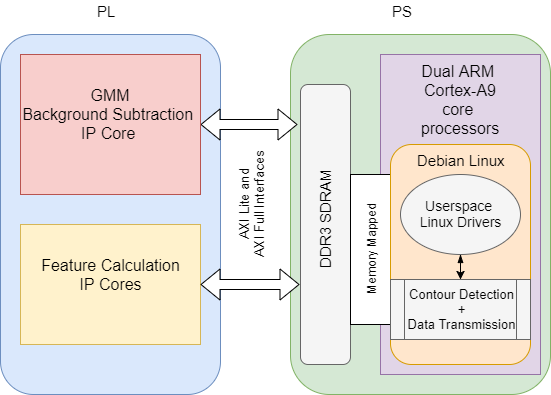
\includegraphics[width=\textwidth]{hardware.png}
\centering
\caption{Architecture of the Leaf node}
\label{leafnode_Archi}
\end{figure}

There are various functions that needed to be executed in the ZYNQ SoC (leaf node). We have the freedom of choice implement these functions in PL or PS. We used the following set of criteria to divide functionality among PL and PS.
If a certain function can be easily parallelized and the latency can be reduced using parallelization and other techniques, that function is implemented in PL
If a certain function is inherently sequential, then it is implemented in PS (Implementing this in PL would not reduce the latency in most cases instead it might even increase the latency)
If the function performs a complex task, it is implemented in PS (Implementing on PL take a long time)
Considering above criteria, we have selected the functions that can be implemented on ZYNQ PL. Table \ref{plvsps} shows the functions implemented on PL side of the ZYNQ and PS side of the ZYNQ.
\begin{table}[H]
\centering
\caption{Implementations on ZYNQ-7000 SoC}
\label{plvsps}
\begin{tabular}{|l|c|c|}
\hline
\multicolumn{1}{|c|}{\textbf{Task}}                                                                       & \textbf{Programmable Logic} & \multicolumn{1}{l|}{\textbf{Processing System}} \\ \hline
\begin{tabular}[c]{@{}l@{}}Video frame capturing \\ from the camera\end{tabular}                          &                             & *                                               \\ \hline
\begin{tabular}[c]{@{}l@{}}Gaussian mixture based \\ background subtraction\end{tabular}                  & *                           &                                                 \\ \hline
\begin{tabular}[c]{@{}l@{}}Morphological operations \\ and people detection\end{tabular}                  &                             & *                                               \\ \hline
\begin{tabular}[c]{@{}l@{}}Feature calculation for \\ people tracking\end{tabular}                        & *                           &                                                 \\ \hline
\begin{tabular}[c]{@{}l@{}}Principal component analysis \\ based false positive elimination\end{tabular}  &                             & *                                               \\ \hline
\begin{tabular}[c]{@{}l@{}}Sending detections and features \\ to central server via Ethernet\end{tabular} &                             & *                                               \\ \hline
\end{tabular}
\end{table}

\subsubsection{IP core implementation on ZYNQ PL}

As mentioned in a previous section, we used a Xilinx High Level Synthesis (HLS) tool called Vivado HLS. High Level Synthesis is an automated design process which converts an algorithmic or a behavioral description to an equivalent digital hardware. Vivado HLS tool is extremely useful in implementing RTL designs using high level implementations of algorithms, quickly and easily. 
Usually using a Hardware Description Language (HDL) such as Verilog or VHDL is the most popular method of designing digital hardware. Compared to designing using HDL, there are few trade-offs in using HLS, which are listed below.
Converting an algorithmic description of a problem to a hardware design is far more easier with HLS than HDL.
Even though there are documentations related to how the high level languages maps to HDL, there is no way to know exactly how the algorithm will be mapped to hardware.
HLS restricts the control over the final hardware design compared to using HDL.
HLS tools are fairly new and still under development compared to HDL tools.
As a personal observation, hardware designs with HLS (Vivado HLS) designed IP cores take less time for synthesis and implementation takes much less time compared to HDL (Verilog) designed IP cores.
Time required for design and optimization with HLS is less than that of using HDL.

IP core design is only a part of out project scope. Considering that and above factors as well as time period allocated for our project, we have decided to use Vivado HLS rather than Verilog (HDL). 


\subsubsection{Gaussian Mixture Model Background Subtraction IP Core}

Gaussian Mixture Model Background Subtraction IP Core is implmented using Vivado HLS tool. Algorithm is explained as follows.\\\\
Gaussian Mixture Models uses a statistical model in which the probability distribution of the luminosity of each pixel is modeled with a mixture of Gaussian distributions. GMM performs really well in identifying the background even in luminosity changes. Our implemented system contains GMM IP core based on the OpenCV GMM algorithm.  The algorithm is optimized for hardware implementation by sectoring the received frame into 60 parts and processing it separately such that the latency and the BRAM utilization is minimized.\\\\
The proposed system models a pixel as a mixture of 2 gaussians. We have limited the system to two models, as a considerable increase of accuracy was not observed by increasing the no of models compared to the increase in resources and latency. A very low latency is desirable for this application as the process needs to be real time. Each model is represented by 4 parameters: mean(µ) , variance(σ2) , weight(w) and Fitness value (F). The weight can be defined as the confidence that a certain gaussian occurs. These parameters differ for each gaussian of each pixel and are updated for every incoming frame of the video.\\
The fitness value is defined as following,

\begin{equation}
F(p,k,t)=\frac{w(p,k,t)}{\sigma(p,k,t)}
\end{equation}

Where $p$ - index of the pixel, $k$ - index of the gaussian distribution and $t$ - frame number. As we employ only two models we compute 2 $F$ values for a single pixel in a frame. The matched condition is checked with the following condition. 

\begin{equation}
M(p,k)=1 \quad \textrm{if}  \quad |pix- \mu(p,k,t)| < 2.5\sigma(p,k,t)
\end{equation}

The above condition checks whether the said pixel can be categorized as a background pixel. As can be seen this condition could be true for more than one gaussian. Thus, the matched distribution is taken as the distribution with the highest F value. The parameters of the matched distribution are updated as follows. 

\begin{equation}
 \mu(p,k,t+1)=  \mu(p,k,t)+ \alpha(pix- \mu(p,k,t))  
\end{equation}

\begin{equation}
\sigma^2(p,k,t+1)= \sigma^2(p,k,t)+\alpha[(pix- \mu(p,k,t))^2-\sigma^2(p,k,t)]
\end{equation}

\begin{equation}
 w(p,k,t+1)=  w(p,k,t)- \alpha w(p,k,t)+\alpha
\end{equation}

$pix$ is the value of the pixel. The learning rate $\alpha$ defines the rate that mean variance and weight are updated. parameters of the unmatched gaussians are not updated. For the first frame $\alpha = 1$, so that the background is initialized from the first frame.  Therefore this algorithm heavily depends on a correct background image being achieved through the first frame.\\\\
If no appropriate gaussian mixture found at all, that is no gaussian distribution for a certain pixel confirms the first condition then the weakest mixture is removed and a new one is created. The weakest mixture is defined as the mixture with the lowest $F$ value.

\begin{equation}
 \mu(p,k,t+1)=  pix
\end{equation}

\begin{equation}
\sigma^2(p,k,t+1)= \sigma^2
\end{equation}

\begin{equation}
 w(p,k,t+1)=w
\end{equation}

$\sigma^2$  is the default variance, $w$ is the default initial weight initialized at 0.05. If no appropriate gaussian is found for a certain pixel then that pixel is categorized as a foreground pixel for that frame. However, if a gaussian satisfies matched condition for a pixel, then that pixel is not straight away assigned as a background pixel. A thresholding condition is checked to see whether the matched gaussian distribution is a background gaussian or not. Fitness values are sorted from maximum to minimum and weights of the respective gaussians are added in succession according to the following equation.

\begin{equation}
\min \sum_{k=1}^{b} w(p,k,t)>T
\end{equation}

Where $T = 0.7$ is the default background ratio. The minimum number of gaussians that satisfies the above equation are categorized as background distributions. If the matched condition of the pixel is satisfied by a gaussian which also satisfies the thresholding condition then it is a background pixel, else it$’$s a foreground pixel.
Top level design of the backgroung subtraction IP core is shown in figure \ref{gmmip}.

\begin{figure}[H]
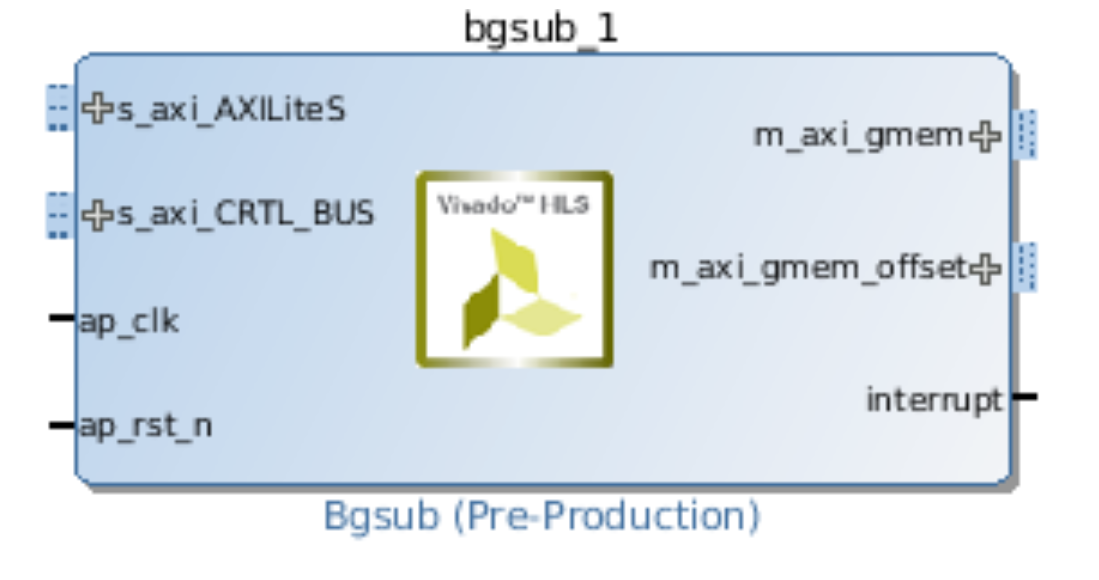
\includegraphics[width=0.8\textwidth]{gmmip}
\centering
\caption{Top level design of background subtraction IP core}
\label{gmmip}
\end{figure}

\subsubsection{Feature Calculation IP Core}

An unique feature for each detected person was needed for tracking each person. We have selected 3D RGB color histogram as the feature based on following criteria,
\begin{itemize}
\item A simple feature with low computational complexity was needed to preserve the real-time nature of the end-to-end system.
\item In the software simulation using above mentioned feature for people tracking, fairly good accuracy was observed. 
\end{itemize}

Figure \ref{hist} shows how the 3D histogram is calculated. Input to the feature calculation IP core is a image frame with each pixel’s RGB components, detected bounding box and background subtracted binary mask.
Algorithm of feature calculation IP core is implemented such that, while iterating through each pixel, it checks two conditions,

\begin{enumerate}
\item Whether current pixel is inside the provided bounding box
\item Whether current pixel is a foreground pixel
\end{enumerate}
If any of the above conditions fail, algorithm moves on to the next pixel. Otherwise that pixel is proceeded through to the next step.\\
In the next step, for each pixel, RGB components are divided by 8. Then these scaled down RGB components are used as the indexes for finding the relevant location of the histogram for that pixel. After relevant coordinate is located on the histogram, it will be incremented by 1.
\begin{figure}[H]
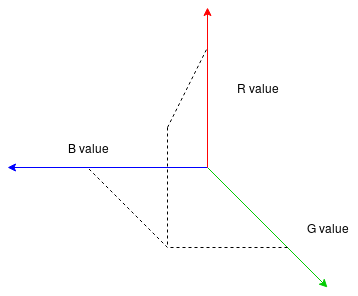
\includegraphics[width=\textwidth]{test.png}
\centering
\caption{Structure of the 3D RGB histogram}
\label{hist}
\end{figure}

Since RGB components of each pixel scaled down by 8, each dimension of the 3D histogram consists of 8 bins (256/8). Therefore result of the above process is a 8x8x8 3D histogram for each detected person. Output of the feature calculation IP core is a 512 element linear array which contains the flattened elements of 3D histogram for the detected person. Figure \ref{featureip} shows a top level block diagram of feature calculation IP core. 
\begin{figure}[H]
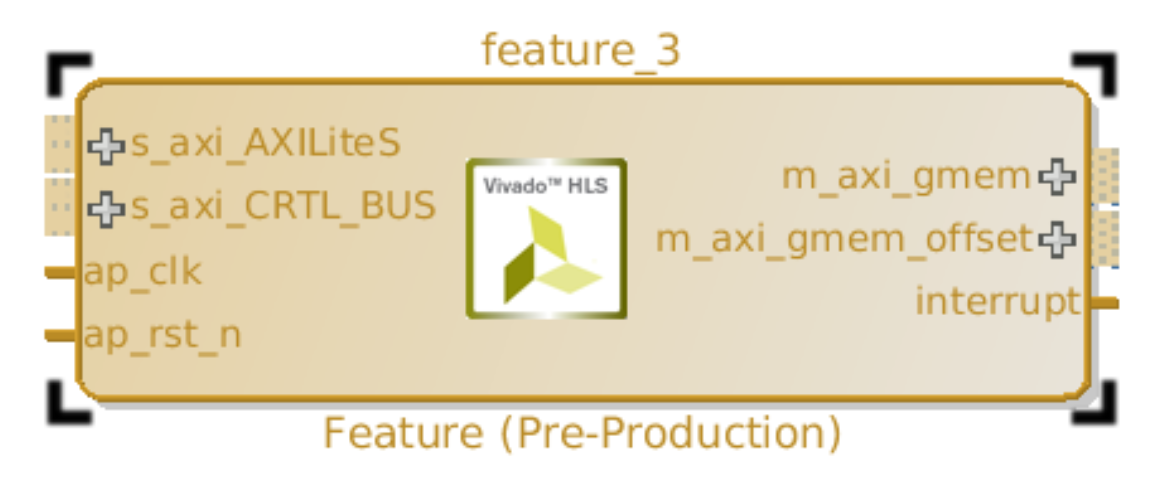
\includegraphics[width=0.8\textwidth]{featureip}
\centering
\caption{Top level design of feature calculation IP core}
\label{featureip}
\end{figure}

\subsubsection{Optimizing Vivado HLS IP Core Designs}
Usually, directly synthesizing C/C++algorithmic designs result in greater resource estimations in Vivado HLS. We have mainly used following two methods for optimizing IP core design in Vivado HLS.
\begin{enumerate}
\item Using compiler directives
\item Dividing all arrays(including video frames) related to the processing into smaller arrays and pipelining at task level
\end{enumerate} 
Vivado HLS provide methods to control the mapping of software description to hardware, to some extent. One of the main method is to use compiler directives provided by Vivado HLS. Every HLS directive starts with \#pragma HLS. Table \ref{pragma} contains the mostly used HLS pragma compiler directives in our designs and brief description about each of them.

\begin{table}[]
\centering
\caption{Vivado HLS Compiler Directives}
\label{pragma}
\begin{tabular}{|l|l|l}
\cline{1-2}
\textbf{HLS Directive Name} & \textbf{Description}                                                                                                                                                                                                                                                     &  \\ \cline{1-2}
PIPELINE                    & Reduces the initiation interval for a function or loop,\\ & by allowing the concurrent execution of operations                                                                                                                                                                &  \\ \cline{1-2}
DATAFLOW                    & Enables task-level pipelining, allowing functions and,\\ & loops to overlap in their operation, increasing the \\ & concurrency of the RTL implementation,\\ & and increasing the overall throughput of the design.                                                                    &  \\ \cline{1-2}
UNROLL                      & Unroll loops to create multiple independent operations\\ & rather than a single collection of,operations. \\ & The UNROLL pragma transforms loops by creating \\ & multiple copies,of the loop body in the RTL design, \\ & which allows some or all loop iterations to occur in,parallel. &  \\ \cline{1-2}
ARRAY\_PARTITION            & Partitions an array into smaller arrays or individual elements.                                                                                                                                                                                                          &  \\ \cline{1-2}
\end{tabular}
\end{table}


\subsection{IP Core drivers and Morphological Operations Implementation on ZYNQ PS}

\subsubsection{Linux Drivers for controlling IP cores}
This was also a challenging task due to the lack of upto date documentation and the complexity of physical memory accessing through Linux kernel. But we managed to overcome this task by using a simple but effective method.\\
When IP cores are generated using Vivado HLS, tool also generates the  following functions, in C language, for controlling the IP core.
\begin{itemize}
\item Starting the IP Core
\item Check whether the IP core is busy or idle
\item Setting input and output addresses
\end{itemize}
But these functions cannot be used directly in the Linux side of ZYNQ PS for controlling the IP cores in the PL, because physical DDR3 memory cannot be directly accessed from Linux OS. Linux only allows the usage of virtual memory in the userspace of Linux OS. 'mmap' function in C++ language was used to overcome this barrier.\\\\
What 'mmap' function does is, it maps a specified region in the physical DDR3 memory onto virtual memory, which can be accessed from the Linux OS userspace level. \\\\
Input/output AXI busses of the IP cores implemented in the ZYNQ PL is mapped onto specific memory locations in the DDR3 RAM. An userspace driver was developed to map these control memory locations and input/output memory locations into virtual memory. Then C functions generated by Vivado HLS were adapted to use these virtual memory to access the physical memory locations relevant to IP cores in an indirect manner. This is shown in figure x as the mapped DDR memory to Debian Linux.
\subsubsection{People Detection from Background Subtracted Binary Mask}

\begin{figure}[H]
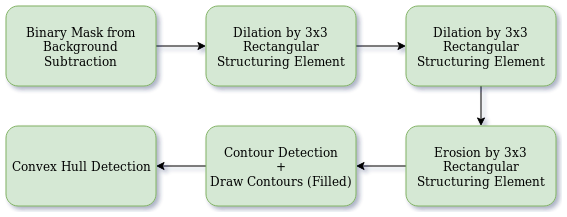
\includegraphics[width=13cm]{morphology.png}
\centering
\caption{Block diagram of the morphological operation flow to detect people from background subtracted binary mask}
\label{morphology}
\end{figure}

Once the background subtracted binary mask is obtained a set of operations are performed as shown in figure \ref{morphology} to enhance the binary image for object detections. 
First a set of morphological operations are performed to clean out the image as necessary. Since the quality of the background model can vary due to various environmental conditions, background subtraction will not give a cleanly filled blob for the shape of a person. There will be a lot of black pixels on the boundary as well as inside the shape of a person. We can use the morphological operation ‘closing’ to fill out these holes. It is essentially two dilations followed by an erosion. Structuring element used here is a 3x3 rectangle. We have tested out several alternatives for the kernel but this kernel size and shape gave the best results for the sequences of images we have tested. Therefore we used it in our final implementation. The results of morphological operations for a test images is shown in figure \ref{fig:sfig3}, \ref{fig:sfig4} and \ref{fig:sfig5}.\\

\begin{figure}
\begin{subfigure}{.5\textwidth}
  \centering
  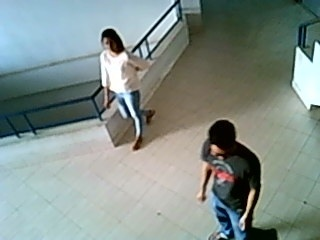
\includegraphics[width=.8\linewidth]{morphology/original.jpeg}
  \caption{Original image}
  \label{fig:sfig1}
\end{subfigure}%
\begin{subfigure}{.5\textwidth}
  \centering
  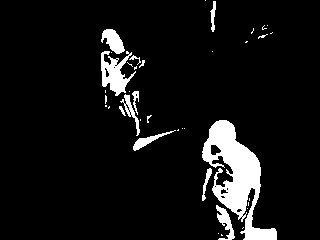
\includegraphics[width=.8\linewidth]{morphology/bgsub.jpeg}
  \caption{Background subtracted binary mask}
  \label{fig:sfig2}
\end{subfigure}\\
\begin{subfigure}{.5\textwidth}
  \centering
  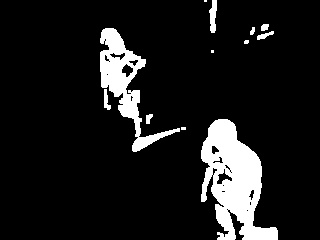
\includegraphics[width=.8\linewidth]{morphology/dilate1.jpeg}
  \caption{Dilation performed on the binary mask}
  \label{fig:sfig3}
\end{subfigure}%
\begin{subfigure}{.5\textwidth}
  \centering
  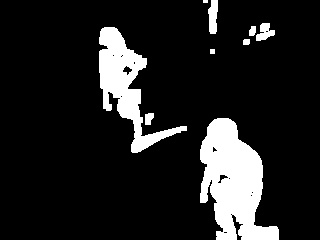
\includegraphics[width=.8\linewidth]{morphology/dilate2.jpeg}
  \caption{Twice dilated}
  \label{fig:sfig4}
\end{subfigure}\\
\begin{subfigure}{.5\textwidth}
  \centering
  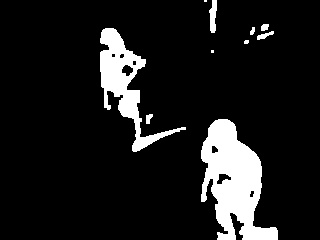
\includegraphics[width=.8\linewidth]{morphology/errode.jpeg}
  \caption{Twice dilated and eroded}
  \label{fig:sfig5}
\end{subfigure}%
\begin{subfigure}{.5\textwidth}
  \centering
  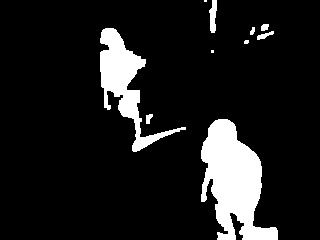
\includegraphics[width=.8\linewidth]{morphology/shape.jpeg}
  \caption{Contour detection and drawing the filled contours taking \ref{fig:sfig5} as input}
  \label{fig:sfig6}
\end{subfigure}\\
\centering
\begin{subfigure}{.8\textwidth}
  \centering
  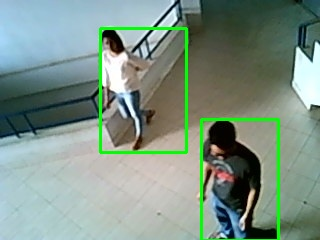
\includegraphics[width=.5\linewidth]{morphology/detections.jpeg}
  \caption{Detecting bounding boxes using convex hull detection}
  \label{fig:sfig7}
\end{subfigure}
\caption{Results of morphological operations for a test image}
\label{fig:fig}
\end{figure}

Morphological operations will give a cleaner image compared to the original background subtracted image. Next contour detection is applied to the output image resulting from morphological operations. We have used inbuilt functions of opencv for this. They have implemented contour detection based on Suzuki’s [7] border following algorithm. Then again using inbuilt functions of opencv we fill out these contours. It will completely fill the shape of the person. The result of this operation for a test image is shown in figure \ref{fig:sfig6}.
\\\\
Next step in this process is to detect the bounding box surrounding the blob of a person. For this we use opencv inbuilt function for convex hull detection. A convex hull is the smallest polygon enclosing a set of points. Opencv’s implementation is based on the algorithm proposed by Sklansky [8]. After this process we obtain a set of bounding boxes corresponding to people detected. Resulting bounding boxes for a test image is shown in figure \ref{fig:sfig7}.

\subsubsection{False Positive Reduction}
Although the above process is able to detect people from an image, it also detects a lot of unwanted blobs due to various reasons such as reflections caused by background surfaces, imperfections of background modeling, etc. Therefore we need to utilize a method to reduce number of these false positives. Our initial approach was to select the bounding boxes satisfying a set of conditions as follows and reject all the other detections.
\begin{itemize}
\item Width of bounding box(w) > TW
\item Height of bounding box(h) > TH
\item TAR1 > Aspect ratio(w/h) > TAR2
\item TCA1 > Contour Area > TCA2
\end{itemize}
Here TW, TH, TAR1, TAR2, TCA1 and TCA2 are constants that are chosen arbitrarily. Initially we tuned up these constants manually by looking at the results. But this was a tedious task and this has to be redone once the camera position is changed. Therefore we explored the possibility of machine learning based automatic way to do this.

\noindent We selected a few features of the bounding boxes into consideration as follows:
\begin{enumerate}
\item Width
\item Height
\item Bounding box area
\item Aspect Ratio (Width / Height)
\item Contour Area
\item Diagonal Length
\end{enumerate}

\begin{figure}[H]
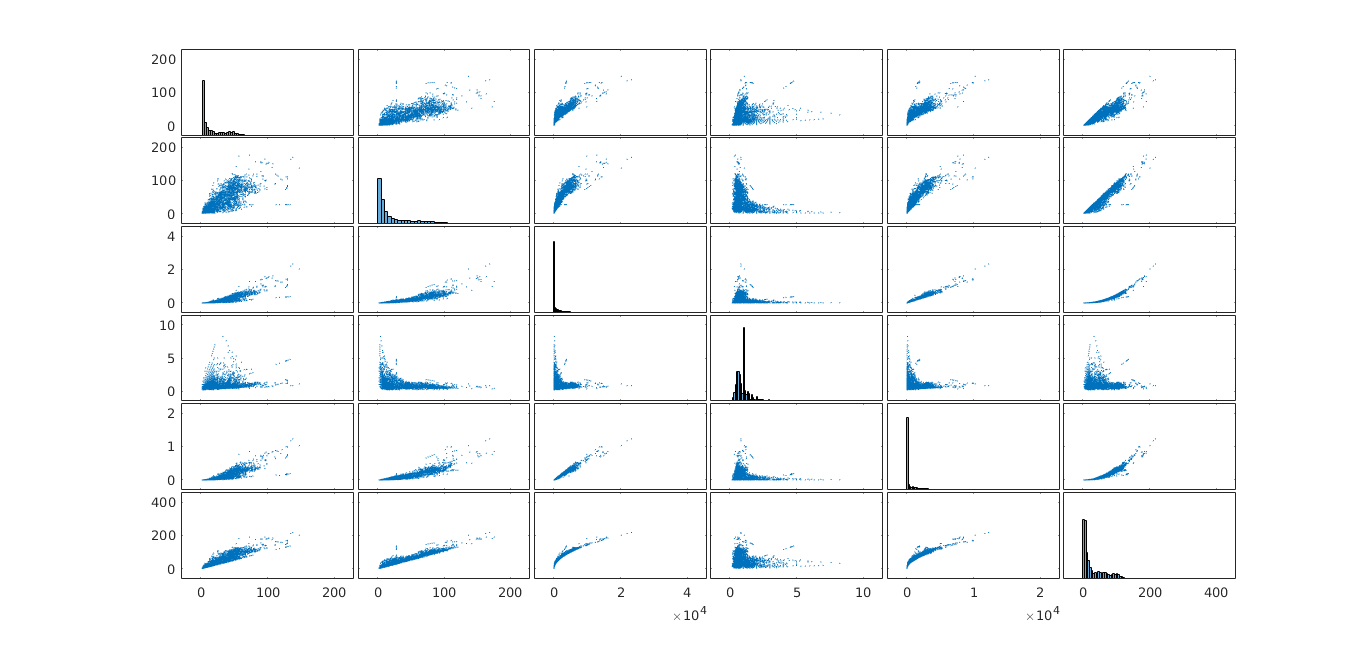
\includegraphics[width=\textwidth]{pca/scatter_plots_pca.png}
\centering
\caption{Scatter plot matrix for the 6 features collected from running our object detection on a sample video}
\label{pca1}
\end{figure}


We can see from the scatter plots above that most of the above features are highly correlated. Therefore we can use Principal Component Analysis to perform dimensionality reduction of the feature space. The percentage of variance explained by each principal component was obtained as follows.\\

\begin{table}[]
\centering
\caption{Percentage of variance along each pricipal component}
\label{pca-table}
\begin{tabular}{|c|c|}
\hline
\textbf{Principal Component} & \textbf{Percentage of Variance Explained} \\ \hline
1                            & 99.4509                                   \\ \hline
2                            & 0.5401                                    \\ \hline
3                            & 0.0063                                    \\ \hline
4                            & 0.0019                                    \\ \hline
5                            & 0.0000                                    \\ \hline
6                            & 0.0000                                    \\ \hline
\end{tabular}
\end{table}

We can see that only the first two principal components give a significant contribution. Even the 2d principal component is less significant compared to the 1st principal component. We can further see this in figure \ref{pca2}.

\begin{figure}[H]
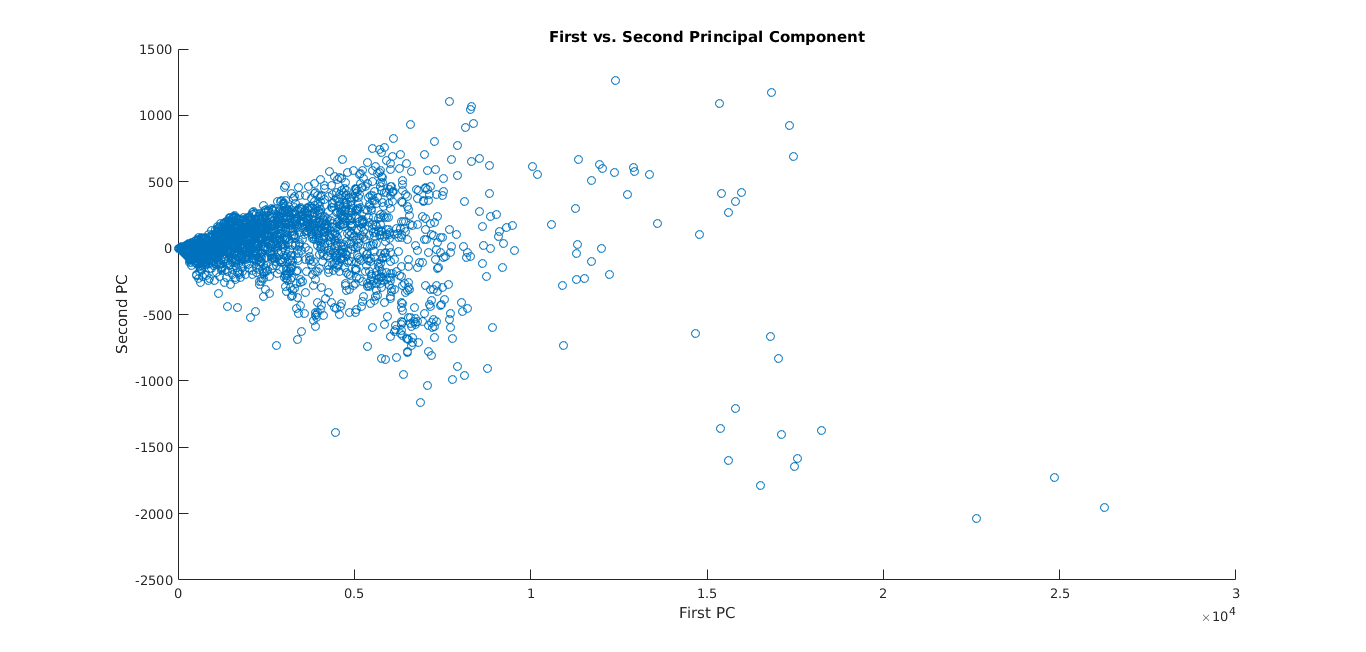
\includegraphics[width=\textwidth]{pca/1_2_pca.png}
\centering
\caption{First Vs. second pricipal component}
\label{pca2}
\end{figure}

\noindent Therefore it is justifiable only to select the first principal component into consideration. 


\begin{figure}[H]
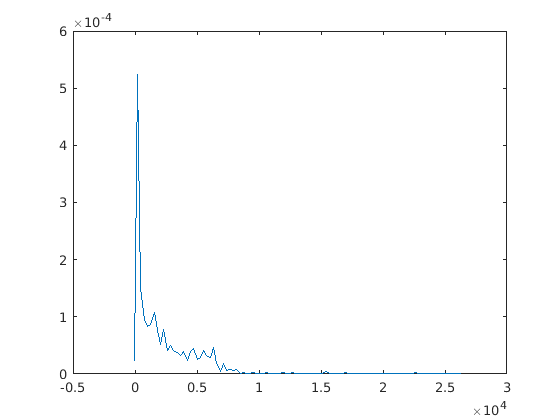
\includegraphics[width=\textwidth]{pca/density.png}
\centering
\caption{Density of the first principal component}
\label{pca3}
\end{figure}

Next we looked at the kernel density estimate of the first principal component as shown in figure \ref{pca3}. We can approximate this with a bimodal distribution. Therefore the problem reduces to finding the optimum threshold for this bimodal distribution. We used Otsu’s [9] thresholding algorithm to find this threshold.
\\\\
We utilized this framework for false positive reduction of the detections. Once we tested out this with several video sequences taken from different camera angles we found out that this method indeed gives better results as analysis suggested. Figure \ref{pca4:pca4} shows the results of PCA based false positive reduction.\\

\begin{figure}
\begin{subfigure}{.5\textwidth}
  \centering
  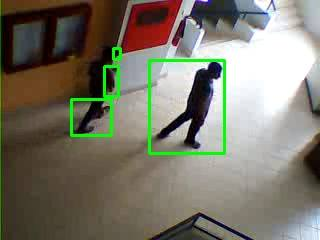
\includegraphics[width=.8\linewidth]{pca/fals_positives.jpg}
  \caption{Raw bounding boxes detected}
  \label{pca4:1}
\end{subfigure}%
\begin{subfigure}{.5\textwidth}
  \centering
  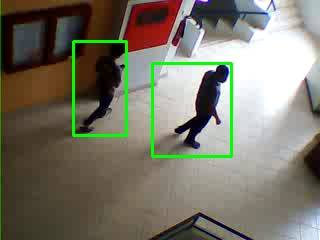
\includegraphics[width=.8\linewidth]{pca/false_positives_eliminated.jpg}
  \caption{With false positive reduction}
  \label{pca4:2}
\end{subfigure}
\caption{Results of PCA based false positive elimination algorithm}
\label{pca4:pca4}
\end{figure}

When applying this method the system should first undergo a training stage where raw detection features are collected. Then coefficients of the first principal component is determined using this dataset. Then the optimum threshold is determined. This whole process was implemented in code so that system can automatically learn to reduce false positives. In the normal mode of operation the system directly uses these calculated coefficients and threshold for false positive reduction.

\subsubsection{Communication Protocol among leaf nodes central server}

Since our system is a multi camera system we need to connect each camera to a central server where people tracking is done. we need to design a communication algorithm to handle the communication between the server and camera nodes. We identified the following requirements for designing such a communication protocol.

\begin{enumerate}
\item Low bandwidth utilization
\item Low latency
\item Scalable with increasing number of cameras
\end{enumerate}

Taking these requirements into consideration we designed a communication algorithm. We used User Datagram Protocol (UDP) to send the data packets, since it has lower overhead and it is also connectionless. In our architecture the backend server will be listening to packets coming from cameras over the network. Each camera node can just start sending data packets to the server at anypoint in time. There is no connecting phase. Server will distinguish packets from different cameras and act accordingly. The advantage of this kind of a setup is we can plugin any camera to the network quite easily and switch it on and start sending data.\\\\
Each datagram sent from a camera will contain the following information.
\begin{table}[H]
\centering
\label{my-label}
\begin{tabular}{|l|l|lll}
\cline{1-2}
Field & Description &  &  &  \\ \cline{1-2}
Camera ID & A number between 0-255 identifying the camera. &  &  &  \\ \cline{1-2}
Time Stamp & Time at which this frame was generated. &  &  &  \\ \cline{1-2}
Detections & Bounding boxes of the detections. &  &  &  \\ \cline{1-2}
Histograms & 512 bin Histograms corresponding to detections. &  &  &  \\ \cline{1-2}
Binary Mask & \begin{tabular}[c]{@{}l@{}}Binary mask obtained from background subtraction is also sent \\ for display purposes.  This can be completely eliminated once the \\ system is deployed.\end{tabular} &  &  &  \\ \cline{1-2}
\end{tabular}
\end{table}

With this information the server can distinguish packets coming from different camera nodes. And also it can identify any missing frames. But in our current implementation we discard missing frames completely. This information is converted into a byte stream using serialization libraries of boost (a c++ library). Then this byte stream is sent to the server through an UDP packet of 49152 bytes. We have chosen this value such that each UDP packet is self contained (i.e. it contain all the information necessary to process the corresponding frame), therefore no fragmentation of UDP packets is necessary.

\subsection{Overall Hardware Architecture on Leaf Node (ZYNQ SoC)}


\begin{figure}[H]
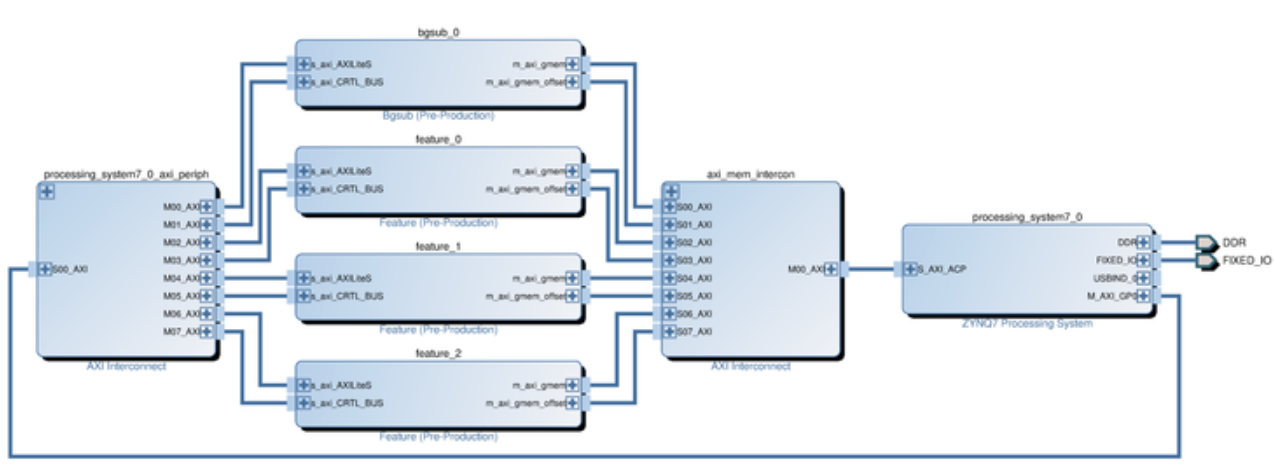
\includegraphics[width=\textwidth]{overallhardware}
\centering
\caption{Overall hardware architecture on Leaf Node}
\label{overallhardware}
\end{figure}


Figure \ref{overallhardware} shows the overall hardware architecture on the ZYNQ-7000 SoC. One background subtraction IP core and three feature calculation IP cores were used in the final design. Each feature calculation IP core can calculate features for only one detected person at a time. Therefore, using multiple feature calculation IP cores, features related to three detections can be done in parallel. All the IP cores are connected to the Accelerator Coherency Port (ACP) on ZYNQ processing system through AXI Full interface. AXI Lite interfaces were used to configure the IP cores, which are connected to Master General Purpose Input/Output (MGPIO) port on ZYNQ processing system. There are two types of memory mapped slave ports on ZYNQ-7000 processing system,
\begin{enumerate}
\item High Performance Ports (HP0, HP1, HP2, HP3) - 32-bit data width
\item Accelerator Coherency Port (ACP) - 64-bit data width
\end{enumerate}
ACP slave port was selected coherency considering the cache coherency issue. This will be explained in more detail in the next section.

\subsubsection{Cache Coherency}

Assume a scenario of two entities sharing a memory and one entity has a local cache. Lets call entity with cache as X and other entity as Y. If the value of a specific memory address is cached by X and Y update the value of that same memory location with a different value without notifying X. In this case, cache of X contains a old (wrong) value.  Cache coherency ensures avoiding these kind of scenarios. 
\par ZYNQ SoC also has a cache coherency issue. PS and PL of ZYNQ SoC share a memory and PS has a local cache. But option of ensuring the cache coherency is only available on ACP port. Therefore, we selected ACP port as the slave on the ZYNQ SoC and manually configured some signals on the port. All bits of following signals on the ACP was set to 1.
\begin{itemize}
\item AWUSER
\item ARUSER
\item AWCACHE
\item ARCACHE
\end{itemize}



\section{Central Server}
In our system, people detection is done at each camera node. Then each camera send this information to the central server. Multi camera people tracking and counting is performed at the central server. This central server perform the following major tasks.
\begin{enumerate}
\item Receiving and unloading data packets from camera nodes
\item Single camera tracking
\item Global multi camera tracking
\item Communication with the web server
\end{enumerate}

\subsection{Receiving and Unloading Data Packets from Camera Nodes}
As mentioned previously we have designed a scalable communication protocol to connect camera nodes to the server. In our implementation we have a UDP server running on a dedicated thread. It listens to any incoming packets through the network. Packets are received, deserialized and pushed into a queue. All the frames in the queue are processed at a interval of 100 ms.

\subsection{Single Camera Tracking}
When it comes to object tracking, detection based tracking methods are the most popular. Multiple object tracking can be decomposed into two parts as, data association and target tracking. These multi object tracking algorithms can be divided into two categories. The first category relies on past frames to estimate the current state recursively. The second category allows for a certain latency and globally solves for all trajectories within a given time window. \\\\
Since our system is to be run in real time, methods under first category are more appropriate for us. Under the first category we tried out Hungary algorithm followed by Kalman Filter based tracker for each object being tracked. As an alternative we tried out particle filter based tracking also. Out of these two we decided to use particle filter based tracking in our implementation due to reasons we will discuss later. 

\subsubsection{Kalman Filter based Tracking}

\begin{figure}[H]
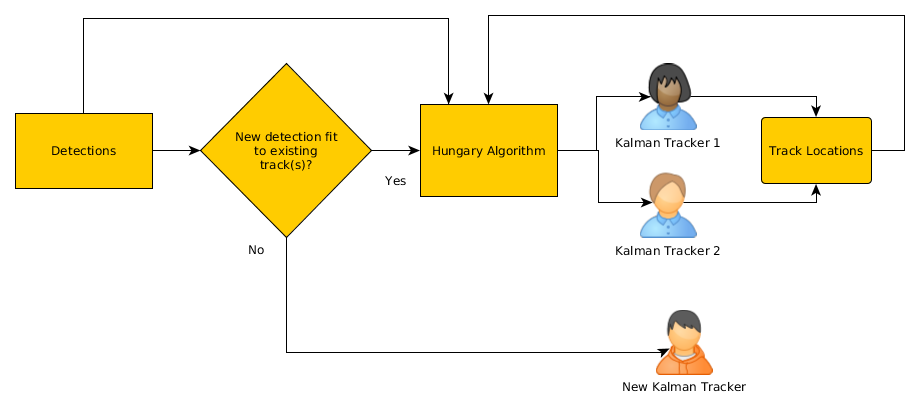
\includegraphics[width=\textwidth]{kalman_hungary_tracker.png}
\centering
\caption{Multiple People Tracking using Kalman Filter}
\label{flask}
\end{figure}
Here detection coordinates are fed to the backend tracking system by individual camera nodes (camera + zynq zc702). The next part of the algorithms calculates a cost matrix for detections vs existing tracks. For m detections and n tracks an entry of the cost matrix is given by equation (3.10).


\begin{equation}
 c_{ij}= cost(detection\ i, track\ j) \quad  where \quad i=1,...,m ; j=1,...,n
\end{equation}

Then detections having the minimum track cost lower than a threshold value are kept and detections exceeding the threshold value are initialized as new tracks. \\\\
Here each track is a kalman filter. Dynamics model used in the kalman filter is a constant velocity model consisting of 6 state variables, namely \string{x coordinate, y coordinate, width, height, x velocity, y velocity\string} and 4 measurement variables, namely  \string{x coordinate, y coordinate, width, height\string}.\\\\
Detections to track assignments are done through the Hungarian algorithm. The Hungarian method is a combinatorial optimization algorithm that solves the assignment problem in polynomial time. Here the individual cost is the euclidean distance between x,y coordinates of the detection and the track. However this can be modified to include the width and height as well.\\\\
Tracks which have not been assigned to a detection within consecutive frames greater than a threshold value are simply deleted. \\\\
Although the kalman filter based tracking gives somewhat satisfactory results, we decided to try out particle filter based tracking also.\\\\
When we look at results we identified several weak points in our current tracking scheme. So we applied some modifications.

\subsubsection{Improvements for Kalman FIlter based Tracking}
In the data association step we have only considered the euclidean distance between detection and tracker coordinates for cost estimation. We improved the accuracy of data association by applying following modifications.

\subsubsection{Gray Level Intensity Histogram as a Parameter in Cost Estimation}
We obtained the gray level intensity histogram for all the detection locations. And we included a histogram parameter in each tracker, where the histogram of the tracker is modified as follows at each assignment of a detection.

\begin{equation}
histogram_{tracker} = \alpha * histogram_{detection} + (1-\alpha) *histogram_{tracker} \quad where \ 0 < \alpha < 1
\end{equation}

Then the correlation between the detection histogram and the tracker histogram is calculated and its inverse $(1/correlation \ coef.)$ is added to the cost. This makes our cost sensitive to the similarity of detection and tracker regions.

\subsubsection{Adding a Penalty for the Cost for High Velocities in Kalman Filter State}

When the kalman filter tends to diverge the velocity value in the state vector becomes high. We can discard the kalman filter quickly by adding a penalty to the cost when the velocity is greater than a certain threshold.

\subsubsection{Tuning model parameters}
We have the following model parameters that must be properly tuned. Currently this is done in an ad hoc manner.

\begin{itemize}
\item Track Initialization Threshold - When the cost exceed this value a new tracker is initialized
\item Rejection Tolerance - When the count of a detection not being assigned to a tracker exceed this value the tracker is deleted
\item Velocity Threshold - Penalty is added to the cost when tracker velocity exceeds this value
\end{itemize}

\subsection{Particle Filter Based Tracking}
\begin{figure}[H]
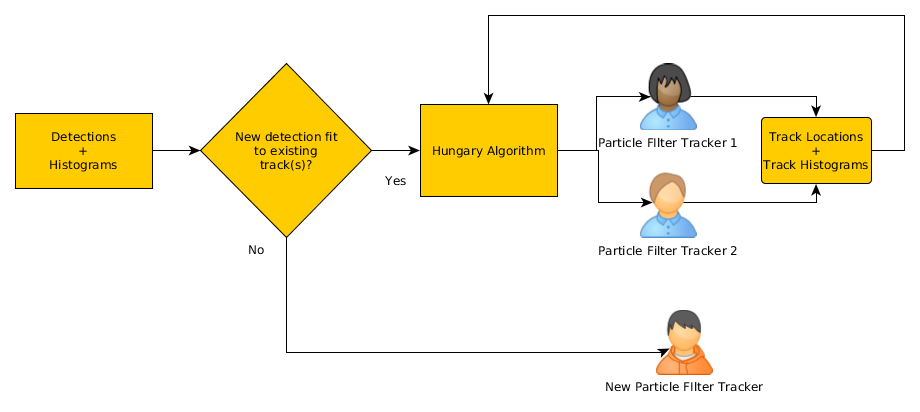
\includegraphics[width=\textwidth]{particle_filter.png}
\centering
\caption{Particle Filter based Tracking}
\label{particle}
\end{figure}

Target tracking system comprising of particle filter trackers are shown in figure \ref{particle}. Arrangement is the same as the one with kalman filter trackers. Only difference is in using particle filter based trackers instead of kalman filter based ones.\\\\
In this setting the particle filter tracks the lower center point of a bounding, which corresponds to the foot of a person. We are using a constant velocity model for particle propagation.  State of a particle consist of 4 states (x, y, vx - velocity in x direction, vy - velocity in y direction). Out of these vx and vy are hidden states. A particle tracker undergoes following 3 stages.
\begin{enumerate}
\item Particle initialization
\item Particle propagation
\item Updating weights with a measurement
\end{enumerate}
In particle filtering sate space is represented as a distribution of particles. Each particle has a weight which corresponds to a probability of this particle being the through location. We will briefly go though his 3 stages of particle filtering.

\subsubsection{Particle Initialization}

A new particle tracker is initialized when a new object is detected for the first time. At this stage x, y are initialized to that of the detection location and vx, vy are initialized to 0. Weight of all the particles are initialized to $1/(no.\ of\ particles)$.

\subsubsection{Particle Propagation}

In this stage particles are propagated according to a constant velocity model. The dynamic model of the system is given equations \ref{eqn:prop1} and \ref{eqn:prop2}.

\begin{equation}
\label{eqn:prop1}
X[t] = X[t-1] + Vx[t-1] * dt
\end{equation}

\begin{equation}
\label{eqn:prop2}
Y[t] = Y[t-1] + Vy[t-1] * dt
\end{equation}
We derive samples from a gaussian distribution to propagate individual particles. Mean of this gaussian distribution is zero with a different variances for 4 states. The 4 variances for x, y, vx and vy are 5.0, 5.0, 1.0 and 1.0.

\subsubsection{Updating Weights with a Measurement}
When a measurement comes the weights of the particles are updated and the particles are resampled according to weights. The weight update equation is as follows.

\begin{equation}
w = \frac{1}{\sqrt{2*\pi* \sigma }}exp\left (\frac{(x_p-x_d)^2+ (y_p-y_d)^2}{2*\sigma }\right )
\end{equation}
Here $x_p$ and $y_p$ are particle locations and $x_d$ and $y_d$ are detection locations. And $\sigma$ is an arbitrary constant.

\subsection{Choosing Particle Filtering over Kalman Filtering}
We implemented both Kalman filtering based tracking and particle filtering based tracking. Then we tracked the same video sequence with both the filters and observed the results. Clearly particle filtering gave better results. And it has the following advantages:
\begin{itemize}
\item Accuracy can be increased by increasing the number of particles (Current implementation consist of 100 particles)
\item More parameters to control compared to the Kalman Filtering
\end{itemize}

\subsection{Data Association}
Data association is an important part of this process because the tracking algorithm performance will be directly depend on the accuracy of data association. For this we utilized the hungarian algorithm. Here we a set of detections having a location and a color histogram, and also a set of tracks having the same. We will assign detections to tracks so that overall cost is minimized. The individual cost is given by equations \ref{eqn:association1},  \ref{eqn:association2} and \ref{eqn:association3}.

\begin{equation}
\label{eqn:association1}
W_d = \frac{1}{\sqrt{2*\pi* \sigma }}exp\left (\frac{(x_t-x_d)^2+ (y_t-y_d)^2}{2*\sigma }\right )
\end{equation}
where $x_t$, $y_t$ are track locations and $x_d$, $y_d$ are detection locations.
\begin{equation}
\label{eqn:association2}
d(H1,H2)=\sqrt{1-\frac{1}{\sqrt{\overline{H_1}\cdot \overline{H_2}\cdot N^2}}\sum_{I}^{ }\sqrt{H_1(I)\cdot H_2(I)}}
\end{equation}
Where $H_1$ is detection histogram and $H_2$ is track histogram and $H_1$ and $H_2$  represents the mean of the histograms. This is known as the bhattacharyya distance [10].

\begin{equation}
\label{eqn:association3}
w = (1-\alpha)*W_d + \alpha*(1-d(H_1,H_2))
\end{equation}
Here $\alpha$ determines the dependence of the cost on the histogram. In the final implementation this was chosen as 0.4.
\subsection{Sensor Fusion}
Once we do single camera tracking for each camera we should synchronize tracks across cameras. Since we use ethernet for the local area network we assumed that network latency is quite low. Therefore we select the latest tracks of each camera for multi camera tracking. Although this method of sensor fusion is quite trivial it is suitable for our current application.

\subsection{Multi Camera Tracking}

Tracking via multiple cameras consist of 3 parts, people tracking per camera, correspondence estimation and global target tracking. There are 2 methods for correspondence estimation: homography based methods and calibration based methods. Homography based methods rely on a set of matched features to calculate homographic transforms between images. Calibration based methods rely on a pre calculated model of the camera.\\\\
Out of these two methods we decided to use calibration based method because it can be easily integrated into single camera tracking algorithms that we considered. We only have to convert individual track coordinates into global coordinates and then perform global tracking.

\begin{figure}[H]
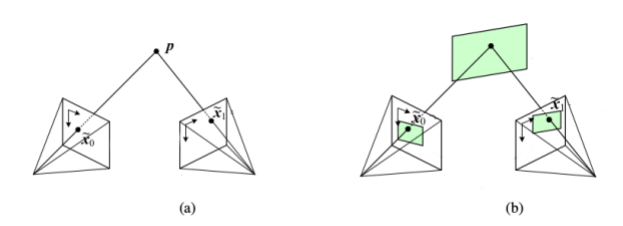
\includegraphics[width=\textwidth]{multi_cam.png}
\centering
\caption{Estimating global coordinates through calibrated cameras}
\label{multi_cam}
\end{figure}
When we have two calibrated cameras as shown in figure (a) the global 3D coordinates can be calculated from the image coordinates obtained from the two cameras, but we have to match the points across the cameras in order to do so. But if we limit our points to an arbitrary plane as shown in figure (b) we can obtain image coordinates projected to that plane. Suppose we limit our points to the ground plane. For this we can multiply the image coordinates (homogenous) by a homography matrix to obtain the ground plane coordinates.
\begin{equation}
x_g = H \cdot x_i
\end{equation}
Where $H$ is a 3x3 homography matrix and $x_i$, $x_g$ in homogeneous coordinates
\begin{figure}[H]
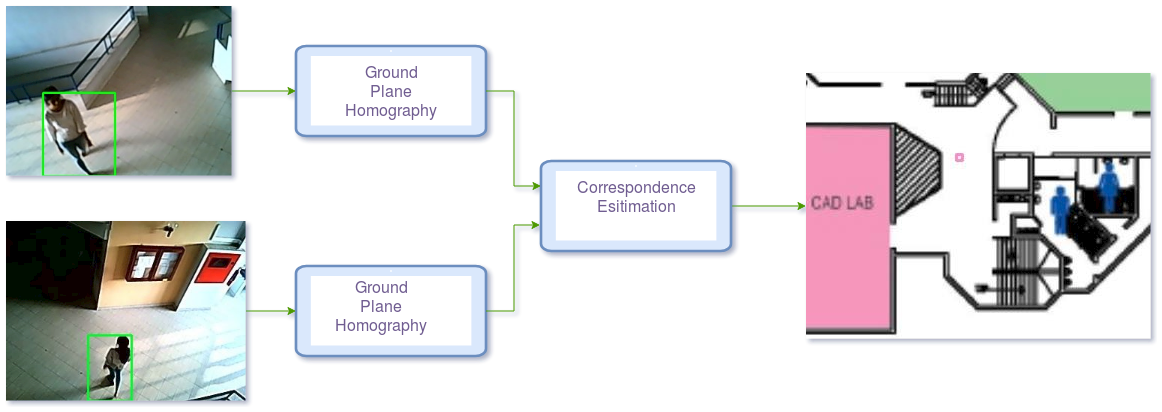
\includegraphics[width=\textwidth]{multi_cam_map.png}
\centering
\caption{Multicamera correspondence estimation}
\label{multi_cam_map}
\end{figure}
Once the image coordinates are transformed to the ground plane we can perform correspondence estimation to find tracks which are seen in multiple viewpoints. For this we can add each track to a node of a graph and join two tracks by an edge if the tracks belong to different cameras and the cost between them is lower than a threshold value.  The cost is calculated by equations \ref{eqn:multicam1}, \ref{eqn:multicam2} and \ref{eqn:multicam3}.

\begin{equation}
\label{eqn:multicam1}
W_d = \frac{1}{\sqrt{2*\pi* \sigma }}exp\left (\frac{(x_a-x_b)^2+ (y_a-y_b)^2}{2*\sigma }\right )
\end{equation}
where a and b are two nodes in the graph.
\begin{equation}
\label{eqn:multicam2}
d(H1,H2)=\sqrt{1-\frac{1}{\sqrt{\overline{H_1}\cdot \overline{H_2}\cdot N^2}}\sum_{I}^{ }\sqrt{H_1(I)\cdot H_2(I)}}
\end{equation}
Where $H_1$ and $H_2$ are the two histograms of nodes a, b and $H_1$ and $H_2$  represents the mean of the histograms. This is known as the bhattacharyya distance [10].
\begin{equation}
\label{eqn:multicam3}
w = (1-\alpha)*W_d + \alpha*(1-d(H_1,H_2))
\end{equation}
Here $\alpha$ determines the dependence on histogram. In our implementation we have chosen $\alpha$ as 0.3. Please note that equations present in here and 3.8.5 have the same mathematics but are used in 2 different settings. Therefore the constants are chosen independently.\\\\
Then we employed a simple greedy algorithm to merge corresponding points together. Here we assuming that cameras have only pairwise overlapping. This algorithm works as follows.
\begin{itemize}
\item Select the edge with lowest cost
\item Merge them together if they have a cost lower than a threshold value
\begin{itemize}
\item Locations are merged by taking the average
\item Histograms are merged by the the combination of two histograms.\\
$H = \beta*H_1 + (1- \beta) * H_2$ Where $\beta$ is selected as 0.5.

\end{itemize}
\item Repeat until edges exist with a cost lower than a threshold value
\end{itemize}
\subsection{Communication with Web Server}
The calculated features are sent to the server, in order to track people and generate business intelligence. To enable communication among FPGA nodes and server we wrote two code structures in C++ and python. C++ client and server snippets connects ZYNQ SoC and the server backend whereas another C++ client and a python server connects the web interface. The block diagram of the communication structure is shown in the figure below.
\begin{figure}[H]
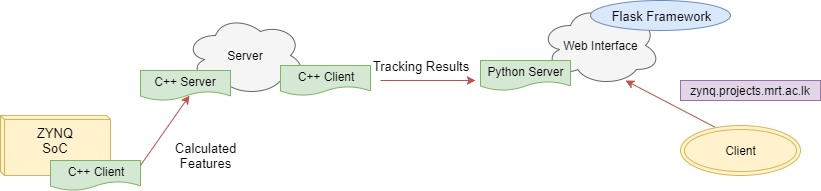
\includegraphics[width=\textwidth]{comm.png}
\centering
\caption{Block Diagram of the Communication Structure}
\label{flask}
\end{figure}
The communications protocol used is UDP (User Datagram Protocol) to ensure low latency and reduce the processing overhead between communication nodes. Since this solution needs to be a real-time application, using TCP (Transmission Control Protocol) is not beneficial. One of the main reasons is dropping packets is desirable over waiting for packets delayed due to retransmission.\\\\
The retrieved features at the server backend are processed and multi camera tracking is done as discussed in the above section, which generates tracking results. Tracking results contain ground plane coordinates of the individuals, track ID and the time stamp at which the data was processed. This information is looped back to the server which is retrieved by a python server and redirects to a web server written on the Flask framework. Flask web framework is based on python and it eases generating business intelligence data.\\\\
Clients can access the web interface through the URL zynq.projects.mrt.ac.lk which directs to an internal server in ENTC. All the processing to generate tracking information is done in the said server. We have acquired a public IP in order to ensure that a client of this product can access the information on the go. Authentication is provided so that unauthorized parties will not be able to access sensitive information.

\subsection{Business Intelligence Software}

Business intelligence software provides the functionality as a website in order to allow access on the go. The web interface is based on Flask web Framework. Flask which is based on Python is ideal for interactive real time user interface which showcases graphical data because Python provides a large graphics library ensuring an aesthetic design pleasing the eyes of the user and conveying the necessary information at the same time effectively.

\begin{figure}[H]
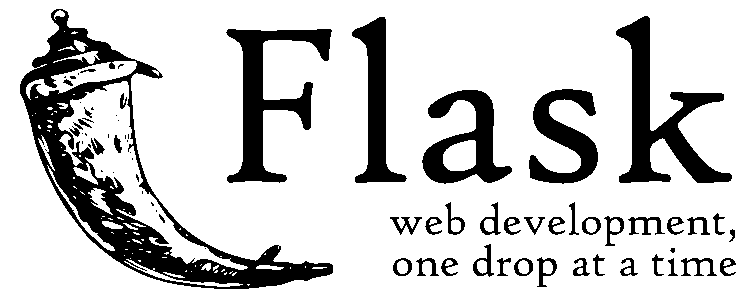
\includegraphics[width=7cm]{flask.png}
\centering
\caption{Flask Logo}
\label{flask}
\end{figure}
To retrieve real time data to the web server we have taken the RESTfull approach, which is based on REST API (Representational State Transfer Application Programming Interface). REST is any interface between two systems which uses HTTP to obtain data and generate operations on those data in a variety of formats, such as XML and JSON. For our design, the web page needs to be constantly updated without reloading the page. That is, the page that generates business intelligence (various graphs) needs to be drawn realtime. To ensure that the data is received realtime without a special user interaction such as pressing a button or refreshing the page we have integrated REST API and AJAX calls which provides the needed functionality.\\\\
Another advantage of the RESTfull approach is that it enables data transfer in JSON object format. JSON is a text-based data format following JavaScript object syntax, which exists as a dictionary which is useful in transmitting data across networks. The data is retrieved to the javascript with AJAX(Asynchronous JavaScript and XML) calls. AJAX calls are important in this scenario because data needs to be sent to the server in the background after the page has been loaded and update it without reloading the page.\\\\
The received data from the server is written to a database to facilitate data storing and retrieval at future time. This is developed with MySQL database platform. Received data is written to two separate tables one to showcase heatmap information and one to provide historical density information. \\\\
All the user credentials are stored in the database in a separate table as well. To access information about his/her store the manager should have user credentials created by the admin team. After successfully logging in only can he access the needed information. Successfully logged in user would be redirected to a URL with generated information about his office.\\\\
Web version of the business intelligence supports 4 formats.
\begin{enumerate}

\item Density - real time store density graph showing the number of customers at the moment.
\item Tracking - real time store map being updated showing the position of each customer at the moment.

\item Heatmap - an interface is provided to enter the starting time and ending time. Heatmap is drawn showing the areas most utilized by the customers during the time period specified. The red color shows high customer density and blue shows relatively low customer density.

\item Historical - when the starting time and ending time is specified customer density over time is drawn for the specified time period. 

\end{enumerate}

This information is vital for an organization in various ways. The number of customers currently browsing the store would be a good indicator to understand how much sales staff should be reassigned to the cashier. Tracking maps could be beneficial to comprehend the customer behavior. Paths customers take while browsing through the store can be recognized and the store can be restructured to provide the ultimate customer experience. If a higher number of customers search for a specific product after selecting another product this could be taken as an indicator that these two products should be placed near to each other. With the heatmap information, a manager would be able to understand customer behavior at different time periods. Which places tend to attract more customers at morning and how should the sales staff be dispersed throughout the store at that time period could be identified. The places that is ideal to showcase advertisements could be identified by looking through these maps. Also at what time advertisements should be shown or promotional activates should take place could be recognized. Historical density data could be utilized into forecasting the number of customers that the store would attract in following days or the same period in the next year. Trends could be analyzed from this data to formulate plans for future. 

\chapter{Results}

\section{Acceleration Using ZYNQ PL}
In an application like this the latency of the system is of utmost importance. To generate the most accurate data people counting and tracking should be done in real-time. As the frequency of obtaining camera frames is very high, the processing speed of the system should be in a high level to process data without any drop of frames. The real-time processing factor could be achieved by reducing the latency as much as possible. 
We ran the proposed people detection algorithm as a software simulation on the ARM processor to compare against the latency we received from implementing the same algorithm in hardware. The resultant latencies and the percentage acceleration that we obtained are shown in the table \ref{accle-table}.
\begin{table}[H]
\centering
\caption{Percentage acceleration by utilizing ZYNQ PL}
\label{accle-table}
\begin{tabular}{|l|c|}
\hline
\multicolumn{1}{|c|}{\textbf{Scenario}}                                                                & \textbf{Average Latency} \\ \hline
\begin{tabular}[c]{@{}l@{}}People detection running on \\ Dual ARM processors in ZYNQ SoC\end{tabular} & 30650us                  \\ \hline
\begin{tabular}[c]{@{}l@{}}People detection running on both \\ PL and PS of ZYNQ SoC\end{tabular}      & 21365us                  \\ \hline
\textbf{Percentage acceleration}                                                                       & \textbf{30.29\%}         \\ \hline
\end{tabular}
\end{table}

As can be seen even though 30\% acceleration was achieved this could be further improved. The main reason for the window of improvement is that we used Vivado HLS in implementing the IP cores for people detection. As the deliverables identified at the initial stage of the project outlined that implementing an end to end system is a must we opted for a smaller design cycle for the FPGA implementation. All the parallelization advantages of FPGA are not utilized at this stage of implementation. However as can be seen by our solution this end to end system providing business intelligence based on leaf node processing at the FPGA is realizable.  Therefore, various optimizations could be done on the system to improve the latency. These could be implemented as future improvements of the system.

\section{Bandwidth Reduction}
 
As we are implementing leaf node processing one of the main results we could achieve was the reduction in bandwidth usage. The received frames are processed at the leaf node to generate bounding box and feature data. Only the x,y coordinates and width and height of the bounding box, track number and features are sent to the server. In other systems whole video frame is sent to the server for detection and tracking.  We have been able to achieve 78.67\% bandwidth reduction with our solution by just sending summarized data. This is a huge reduction in bandwidth usage that we have achieved.

\section{Overall Hardware Utilization}
Table \ref{uti1} shows the number of resources available on ZYNQ PL (resources of XC7z020 FPGA). Figure \ref{util2} shows the percentage utilization for our overall design on ZYNQ PL. This includes one background subtraction IP core and three feature calculation IP cores.
\begin{table}[H]
\centering
\caption{Total resources on ZYNQ PL (Xilinx XC7z020 FPGA)}
\label{uti1}
\begin{tabular}{|l|c|}
\hline
\multicolumn{1}{|c|}{\textbf{Resource}} & \textbf{Amount} \\ \hline
Logic cells                             & 85K             \\ \hline
Look-Up Tables (LUTs)                   & 53 200          \\ \hline
Flip-Flops                              & 106 400         \\ \hline
Total Block RAM                         & 4.9 Mb          \\ \hline
DSP Slices                              & 220             \\ \hline
\end{tabular}
\end{table}


\begin{figure}[H]
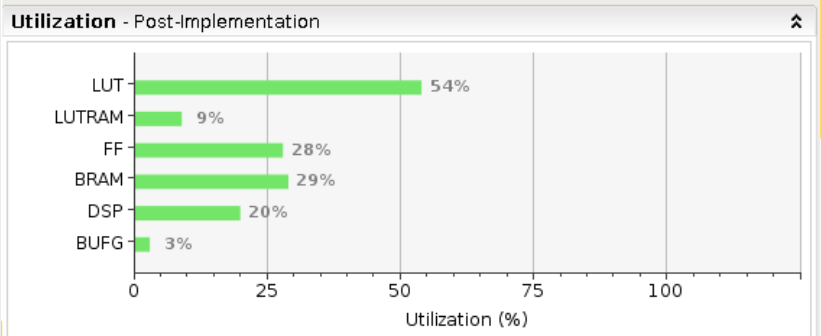
\includegraphics[width=10cm]{utilization.png}
\centering
\caption{Percentage resource utilization of the system on ZYNQ PL}
\label{util2}
\end{figure}




\section{Total on Chip Power}
Figure shows the power estimates generated by Vivado tool for our overall design.
\begin{figure}[H]
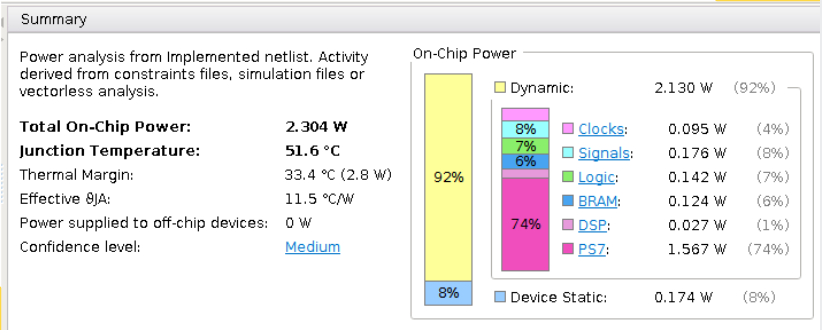
\includegraphics[width=10cm]{power.png}
\centering
\caption{Power estimation of the overall system on ZYNQ SoC}
\label{flask}
\end{figure}

\section{Detection Accuracy}
Detection accuracy is vital in understanding the precision of the system. The whole system depends on how accurately it can identify a person in the frame. Tracking information gets affected by the detection accuracy since if it cannot correctly detect a person the generated tracking information would be wrong from the beginning.
We have tested our detection accuracy against multi camera datasets available. The data set we used is EPFL dataset for multi-camera and pedestrian videos. The camera sequences feature several synchronized video streams filming the same area under different angles. The cameras are located about 2 meters from the ground. We also tested our algorithm for a video frame set that we captured at the ENTC 3rd floor. This video set was obtained by placing two overhead cameras.
Table \ref{accuracy} showcases the results we have obtained for those test data.
\begin{table}[H]
\centering
\caption{Accuracy of People Detection for Various Datasets}
\label{accuracy}
\begin{tabular}{|l|c|c|c|}
\hline
\multicolumn{1}{|c|}{\textbf{Dataset}} & \textbf{False positives} & \textbf{False negatives} & \textbf{Accuracy} \\ \hline
EPFL dataset- terrace                  & 10.4\%                   & 15.1\%                   & 74.5\%            \\ \hline
EPFL dataset - campus                  & 8.5\%                    & 20.3\%                   & 71.2\%            \\ \hline
EPFL dataset - passageway              & 5.2\%                    & 14.3\%                   & 80.2\%            \\ \hline
Our dataset                            & 1\%                      & 10.2\%                   & 88.8\%            \\ \hline
\end{tabular}
\end{table}

False positives occur when the algorithm detects a person in the frame, when there is no person present. False negatives occur when the algorithm fails to detect a person who is really in the frame. 
As can be seen in the above table the highest accuracy is shown for our dataset which has 88.8\% accuracy. The reason for this is that when obtaining the camera feeds, we used overhead cameras. For the EPFL dataset the cameras are mounted 2 meters from the ground. Our algorithm is implemented assuming the cameras are located overhead and the occlusions are minimal. Therefore, the results we achieved are satisfactory. 
The detection accuracy could be further improved by implementing a more sophisticated algorithm in the FPGA. For that we need to go for a FPGA with enhanced features.


\section{Business Intelligence Software}
The subsequent offering of the system is business intelligence software which comes in two versions.  one as a website for the managers and one as a QT GUI application for the admins of the system. 
Web version of the business intelligence supports 4 formats that is density, tracking, heat-map, historical. The interface of the website is shown in figures \ref{web:1}, \ref{web:2}, \ref{web:3} and \ref{web:4}. Graphs generated by the website is shown in figures \ref{graph1} and \ref{graph2}.


\begin{figure}[H]
  \centering
  
\includegraphics[width=.8\linewidth]{web1}
  \caption{Welcome and introduction to the site}
  \label{web:1}
\end{figure}
\begin{figure}[H]
  \centering
  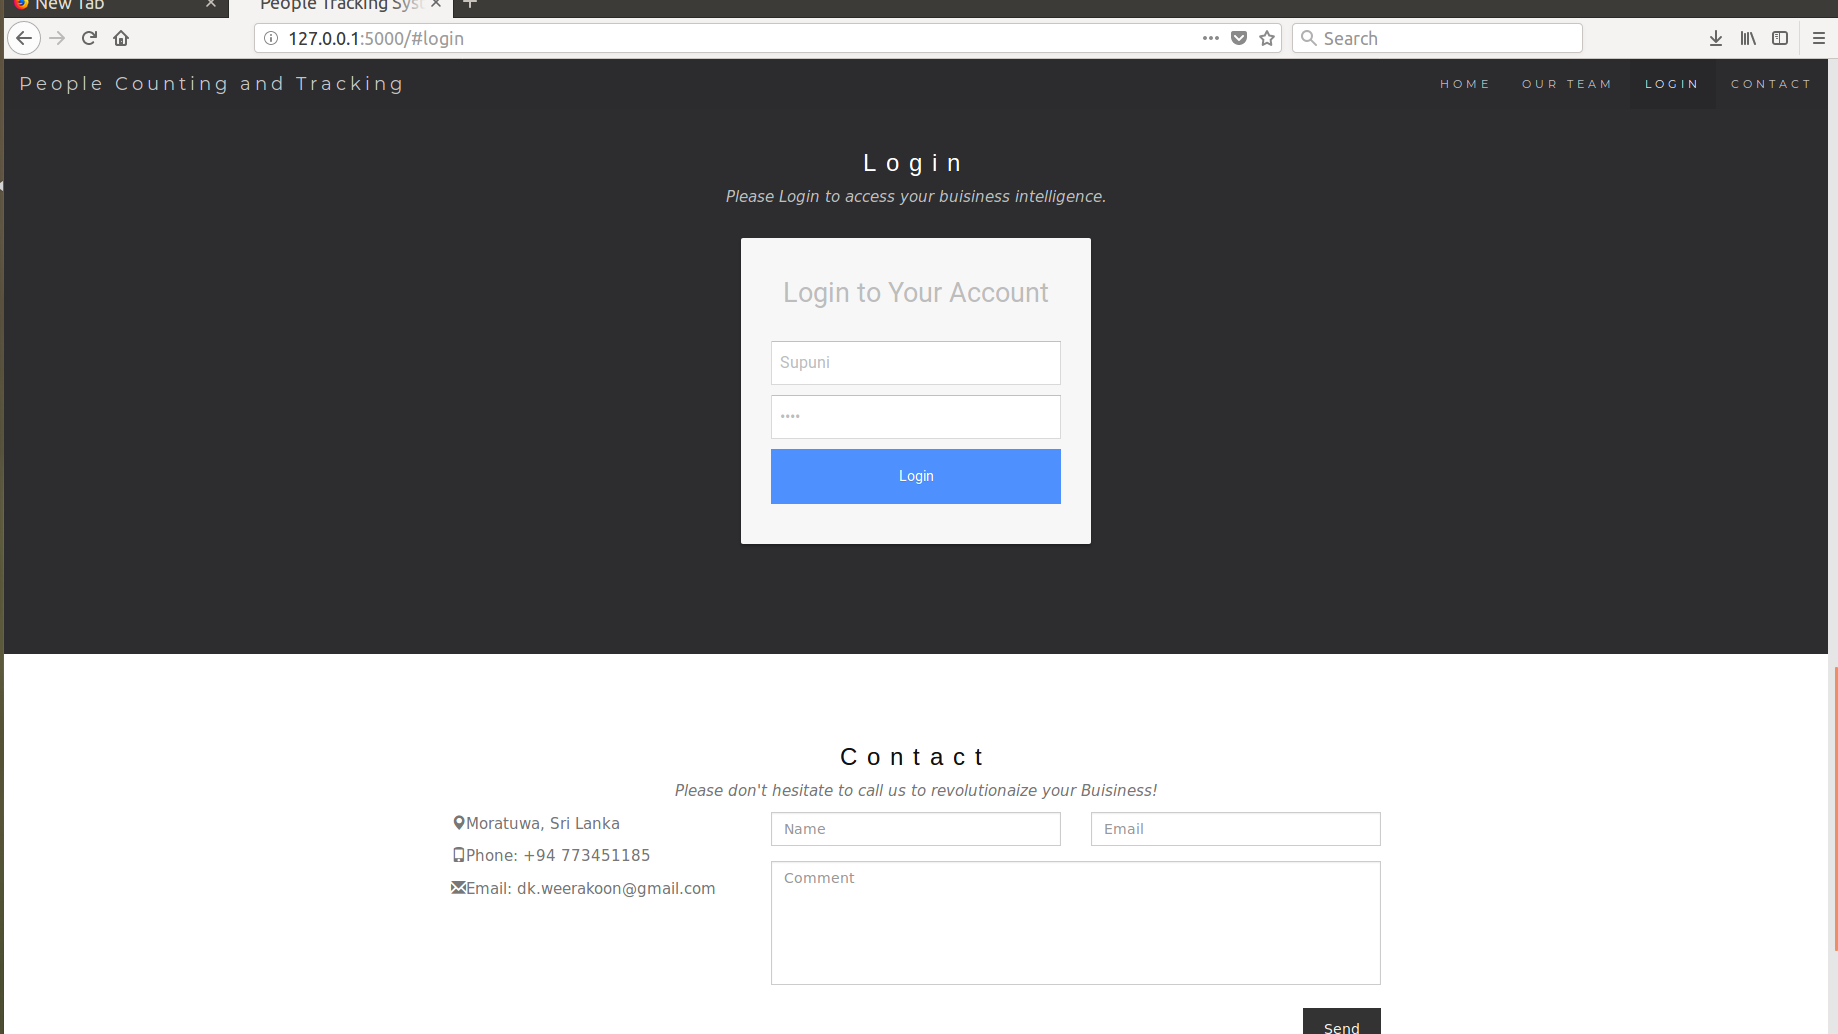
\includegraphics[width=.8\linewidth]{web2}
  \caption{Login prompt for the user}
  \label{web:2}
\end{figure}
\begin{figure}[H]
  \centering
  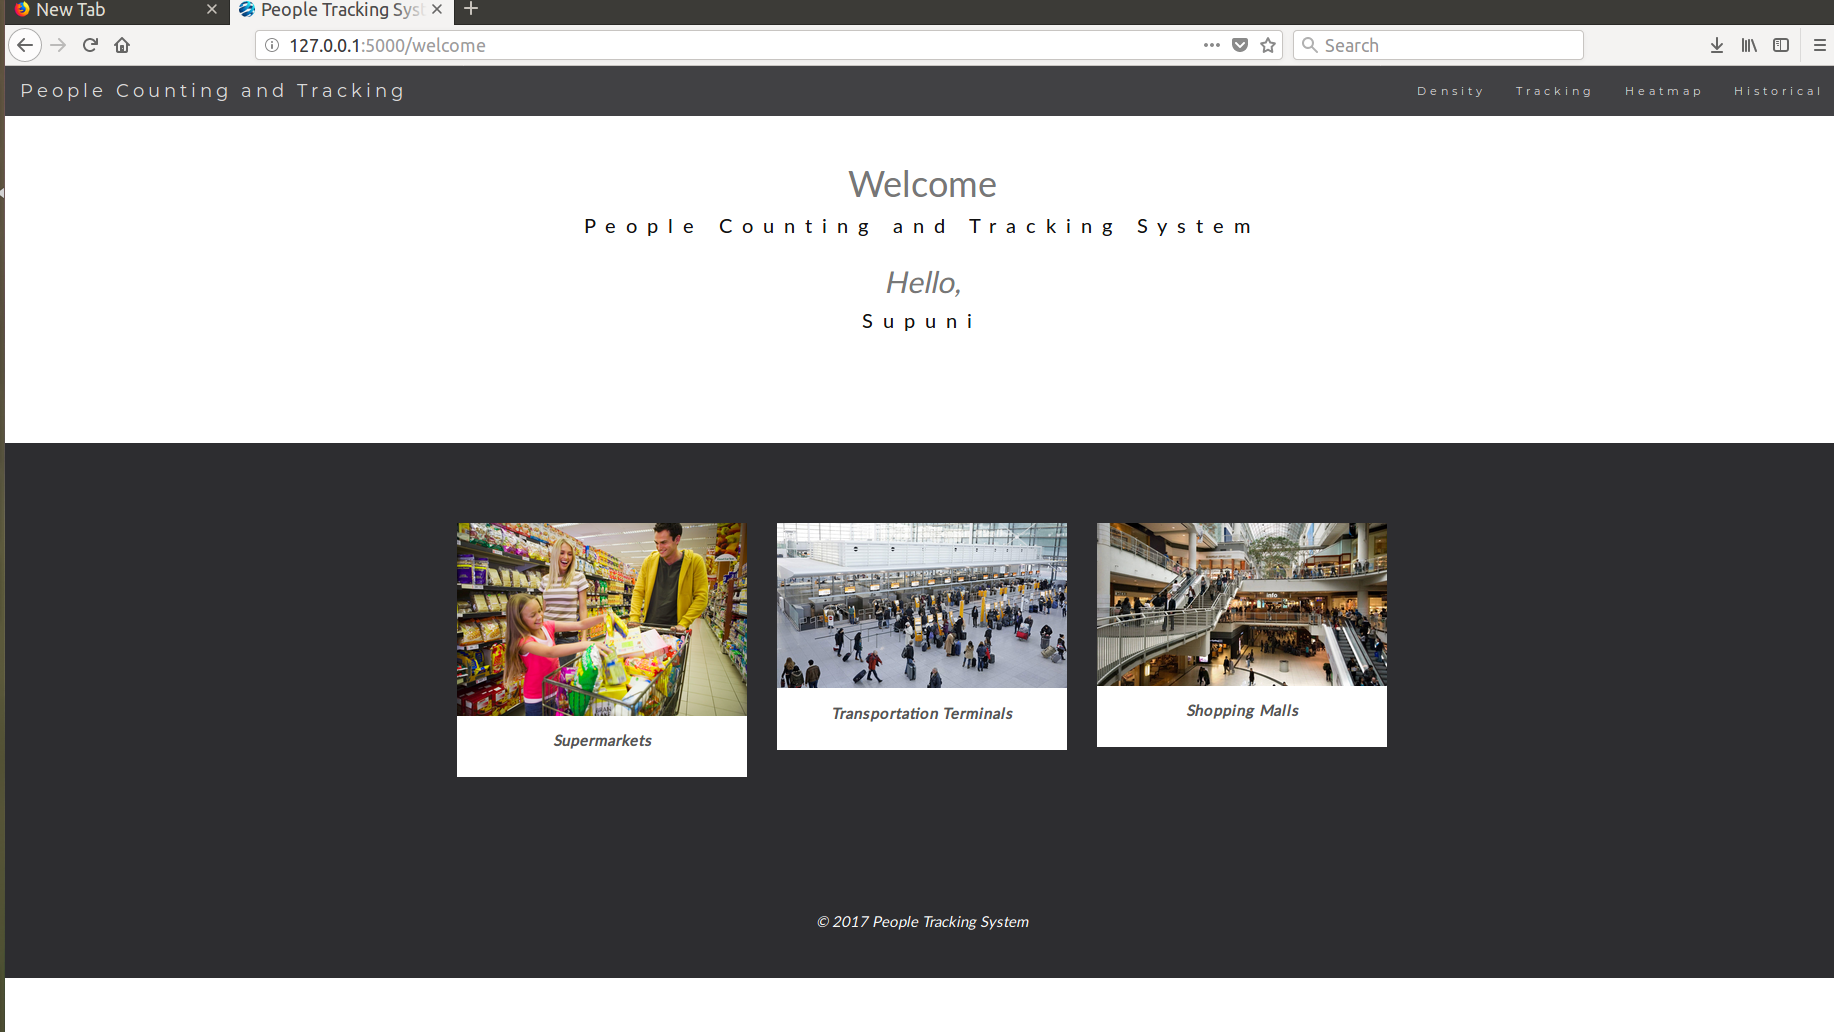
\includegraphics[width=.8\linewidth]{login}
  \caption{Choices for a logged user}
  \label{web:3}
\end{figure}
\begin{figure}[H]
  \centering
  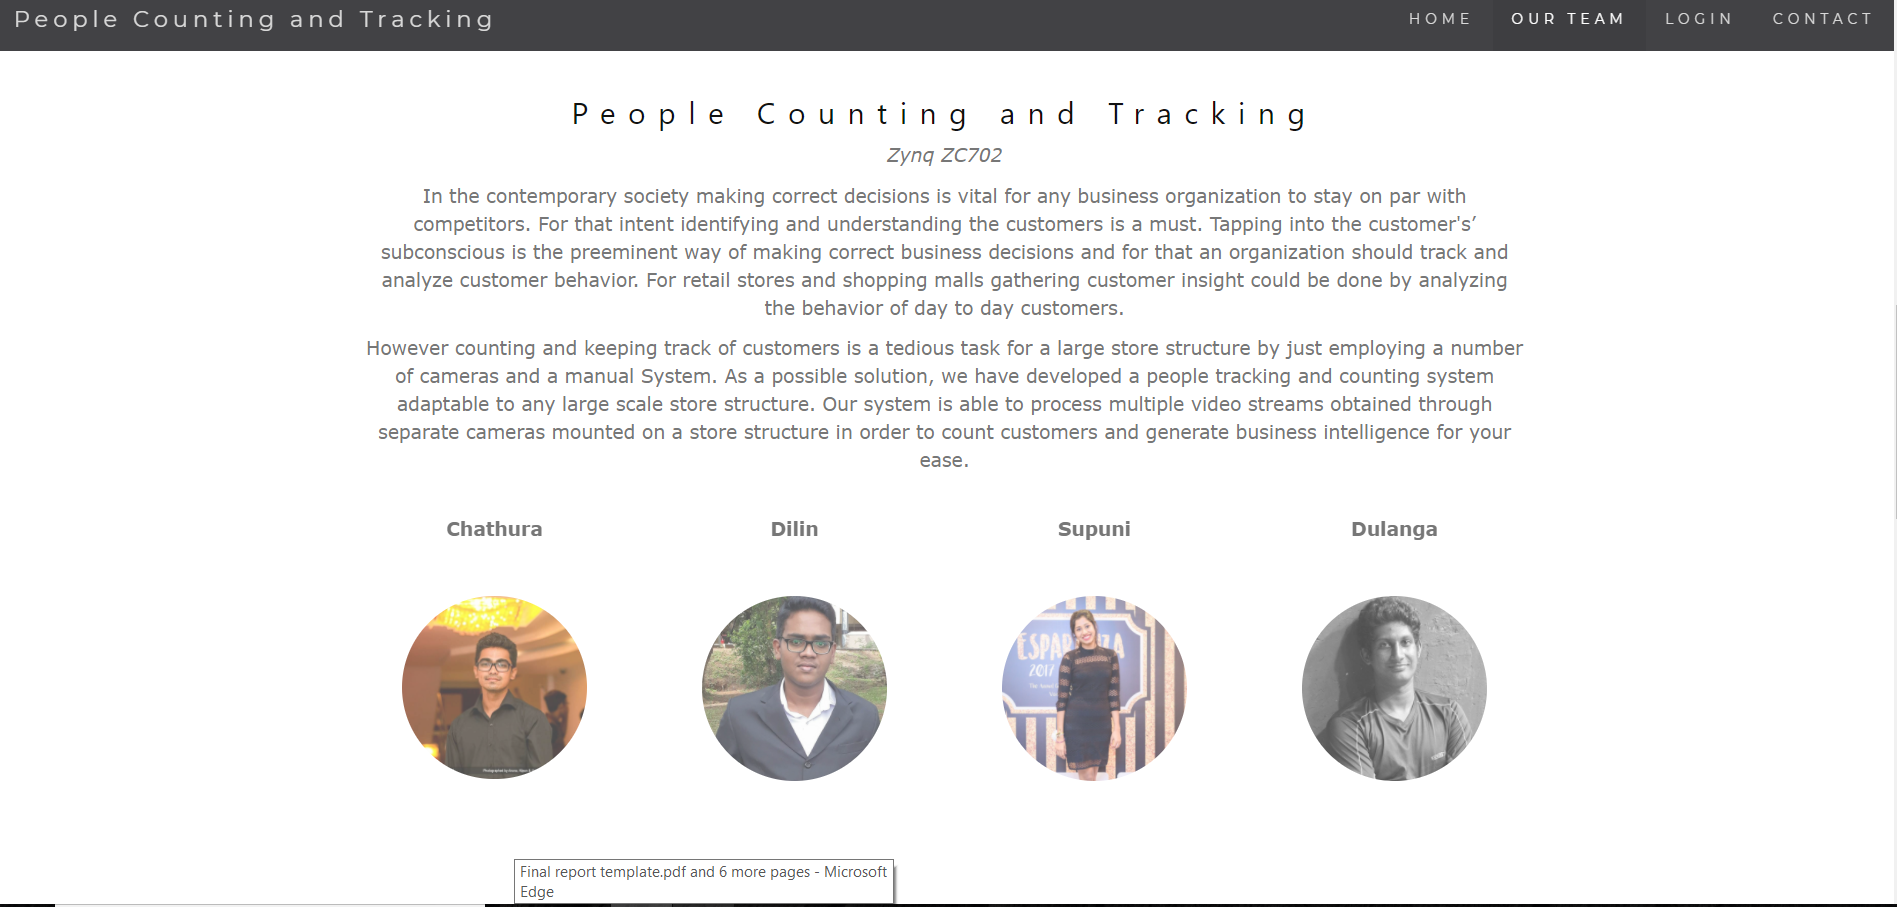
\includegraphics[width=.8\linewidth]{Capture}
  \caption{Design team of the project}
  \label{web:4}
\end{figure}

\begin{figure}[H]
  \centering
  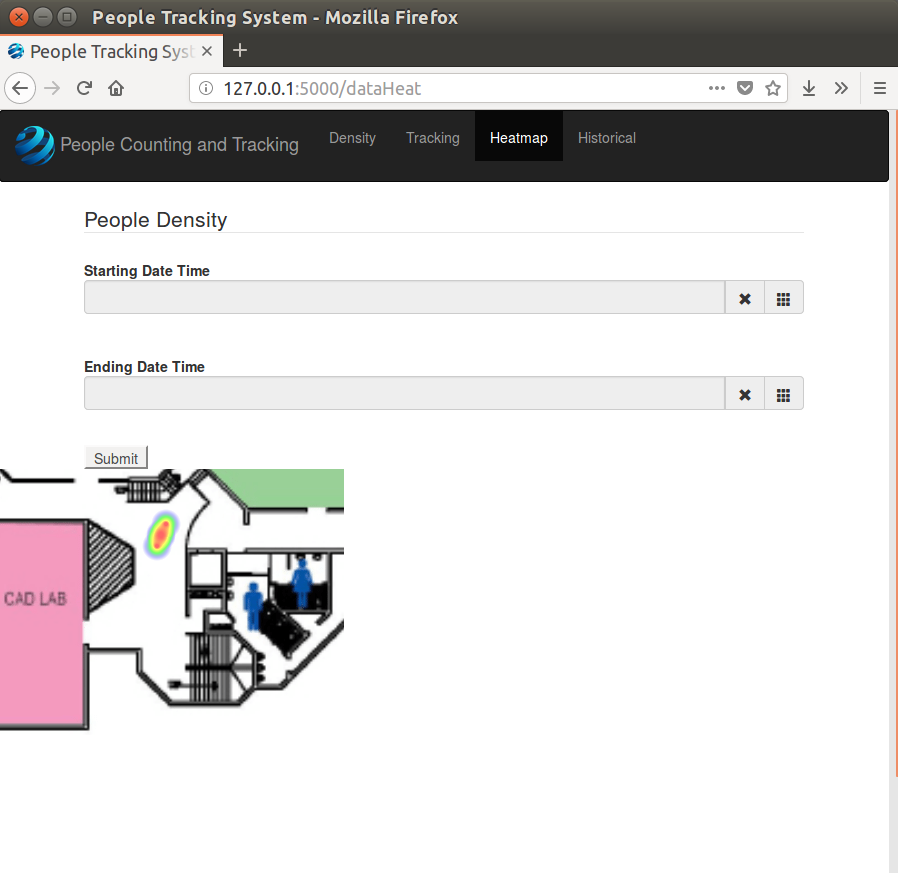
\includegraphics[width=.6\linewidth]{heatmap}
  \caption{Heat-map generated by the web interface}
  \label{graph1}
\end{figure}
\begin{figure}[H]
  \centering
  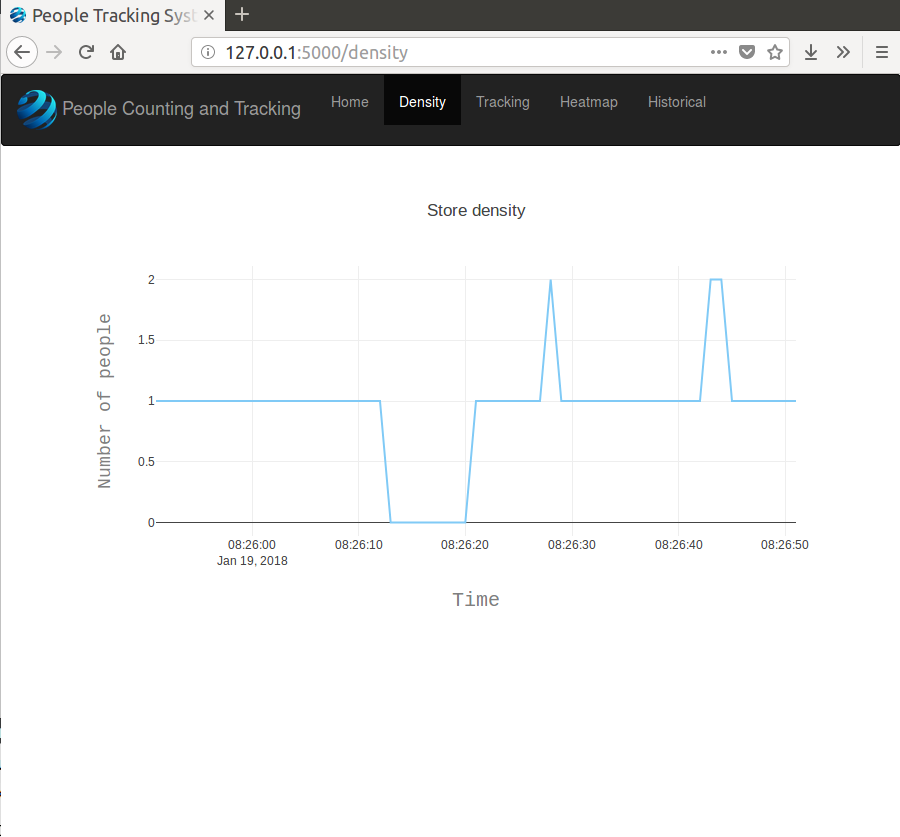
\includegraphics[width=.6\linewidth]{density}
  \caption{People density graph generated by the web interface}
  \label{graph2}
\end{figure}
\newpage
\section{Conclusion}

For a business organization to stay on par with their competitors, understanding their customers is a must. This project provides a solution to that problem by processing the already available data in an intelligent manner and providing business insight to aid in making management decisions. Proposed system is scalable unlike most of the similar systems available in the market today.\\
\par Leaf node processing is a novel approach that we introduced for people tracking. The systems in use today provides people tracking, but scalability issue comes into play in those systems. The main reason is those systems aggregate all the camera feeds to a central server and process the frames in the server. The scalability is largely limited by the processing power of the server. In our solution scalability was achieved by employing a node processing system which utilizes a FPGA + ARM Processor at the leaf node for the people detection. By distributing some of the processing to the leaf node we have been able to realize scalability to a large extent. Currently we have designed our system for 2 cameras. However, it is just a matter of installing another camera and FPGA + ARM Processor in the store to extend the system. Processing power of the server does not affect the functionality of the system at all.\\
\par A palpable reduction in bandwidth usage was also seen as much as 78\% through the architecture of our system. This reduction in bandwidth is achieved by processing the raw video frames at the node itself and only sending the processed data to the server. People detection is done at the leaf node which results in bounding box and features for each detected person.  Only this information being sent to the server against sending the whole frame to the server reduces the bandwidth requirements drastically. \\
\par The scope of this project was to implement a scalable end to end system for Multi-Camera People Tracking utilizing a Zynq SoC for leaf node processing. We have successfully achieved the goals we set at the beginning of the project thereby using an FPGA + ARM processor for leaf node processing, software running on a central server for multi-camera people tracking and a web application (deployed on a web server) for generating business intelligence. Because of the scale of the deliverables, we had to choose a design cycle which would consume a short time to implement the people detection part. Therefore, Vivado HLS was used to implement background subtraction IP core and Feature IP core. FPGA based hardware parallelization was not utilized to the full extent because it is difficult to control the level of parallelization with Vivado HLS. However, as the system is implemented now and since we know that this task is possible in FPGA future optimizations and improvements could be done to advance the performance of the system.\\
\par Our people detection framework is based on contour detection of the background subtracted binary image obtained by the Gaussian Mixture Model. But if we just utilize this framework it gave a lot of false positives. Therefore we came up with came up with a principal component analysis based machine learning algorithm that can train the system to reject false positives.\\
\par Although people detection algorithm performs acceptably, the detection accuracy can be improved further by implementing a better feature extracting algorithm and a sophisticated algorithm for people identification. This implementation would aid in paving the path way for people re-identification as well, which is not currently implemented. If a person goes out of the frame in the system and comes back again, a new track is assigned, whereas a unique track ID is assigned as long as he is in the camera viewpoints. People re-identification is identifying a person who went out of the camera view points and came back as the same person and assigning him the same ID. People re-identification aids in uniquely identifying a person and understanding the shopping behavior of the customers by correctly identifying the paths that one person takes through the shop.\\
\par One of the major issues in single camera tracking is solving the nonlinear data association problem. In our initial implementations we used euclidean distance between detection and tracker coordinates to perform data association. But when there are several detections in close vicinity invalid assignments are obtained. In order to overcome this we made several modifications to our original algorithm. As a major modification we incorporated a weighted average of distance based cost and color histogram similarity based cost, to calculate costs for the Hungarian algorithm, which performs data association. Also we decided to use particle filter based tracking to track the location of foot of a person. These improvements made it possible to track people with a considerable accuracy.\\
\par In implementing the multi camera tracking algorithm we assumed our cameras are static, i.e. their orientation and position would not change with time. Then we calculated a homography that maps ground plane points in the image to a floor map. Next challenge was to develop an algorithm that will estimate the correspondence between detections made my multiple cameras. For this we developed a greedy correspondence estimation algorithm.\\

\par This was a challenging project because the scope was large. But we tackled all the challenges we faced throughout the project successfully and we were finally able to implement a deployable system. 




\newpage
%\section*{\textbf{References}}
\addcontentsline{toc}{section}{References}
\begin{thebibliography}{10}

\bibitem{1}
Vicente, Alfredo Gardel, et al. "Embedded vision modules for tracking and counting people." \textit{IEEE Transactions on Instrumentation and Measurement} 58.9 (2009): 3004-3011.

\bibitem{2}
Dalal, Navneet, and Bill Triggs. "Histograms of oriented gradients for human detection." Computer Vision and Pattern Recognition, 2005. CVPR 2005. \textit{IEEE Computer Society Conference on}. Vol. 1. IEEE, 2005.

\bibitem{3}
Negi, Kazuhiro, et al. "Deep pipelined one-chip FPGA implementation of a real-time image-based human detection algorithm." \textit{Field-Programmable Technology (FPT), 2011 International Conference on}. IEEE, 2011.

\bibitem{4}
Redmon, Joseph, et al. "You only look once: Unified, real-time object detection." \textit{Proceedings of the IEEE Conference on Computer Vision and Pattern Recognition}. 2016.

\bibitem{5}
Andriyenko, Anton, Konrad Schindler, and Stefan Roth. "Discrete-continuous optimization for multi-target tracking." \textit{Computer Vision and Pattern Recognition (CVPR), 2012 IEEE Conference on}. IEEE, 2012.

\bibitem{6}
Tang, Nick C., et al. "Cross-camera knowledge transfer for multiview people counting." \textit{IEEE Transactions on image processing} 24.1 (2015): 80-93.

\bibitem{7}
Yang, Tao, et al. "Robust people detection and tracking in a multi-camera indoor visual surveillance system." \textit{Multimedia and Expo, 2007 IEEE International Conference on}. IEEE, 2007.

\bibitem{8}
Flask.pocoo.org. (2017). Tutorial — Flask Documentation (0.12). [online] Available at: http://flask.pocoo.org/docs/0.12/tutorial/ [Accessed 6 Oct. 2017].

\bibitem{9}
Pythonprogramming.net. (2017). Python Programming Tutorials. [online] Available at: https://pythonprogramming.net/flask-registration-tutorial/ [Accessed 6 Oct. 2017].

\bibitem{10}
Flask-restful.readthedocs.io. (2017). Flask-RESTful — Flask-RESTful 0.3.6 documentation. [online] Available at: https://flask-restful.readthedocs.io/en/latest/ [Accessed 6 Oct. 2017].
\end{thebibliography}


\end{document}